\section{Initial Project Idea}\label{appendix:initIdea}
\begin{figure}[!htbp]
    \centering
    \noindent\begin{subfigure}[b]{\textwidth}
        \centering
        \frame{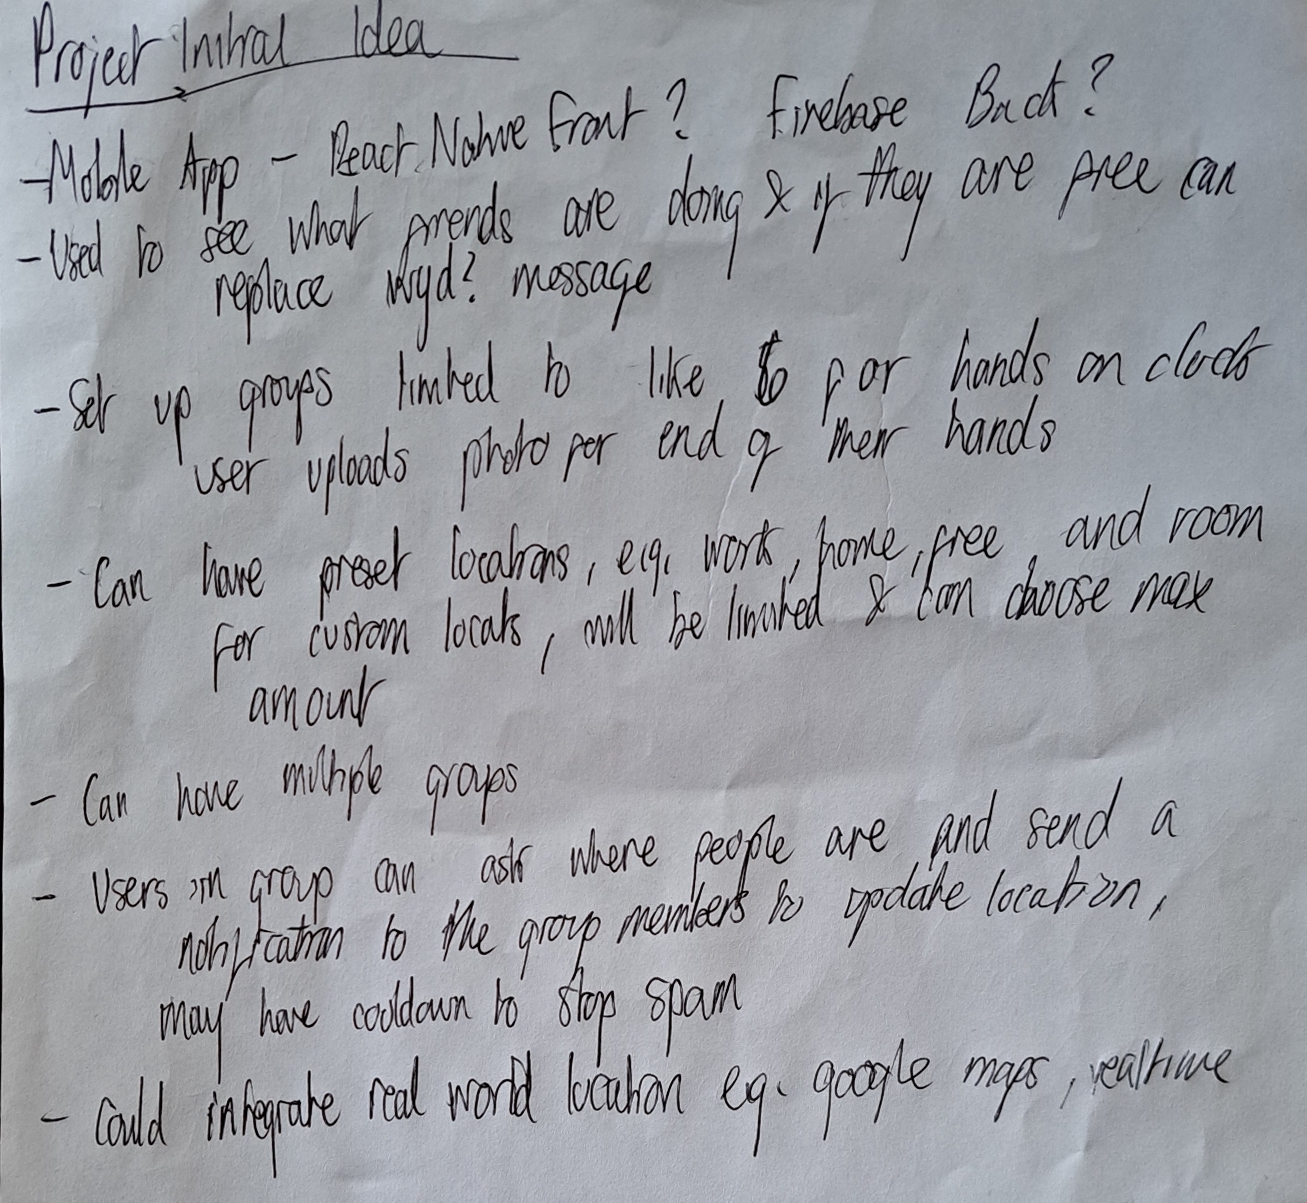
\includegraphics[width=\textwidth]{initialProjectIdea.jpg}}
    \end{subfigure}
\caption{Initial Project Idea}
\end{figure}
\FloatBarrier
\newpage


\section{Figma Designs}\label{appendix:figmaScreens}
\begin{figure}[!htbp]
    \centering
    \noindent\begin{subfigure}[b]{0.23\textwidth}
        \centering
        \frame{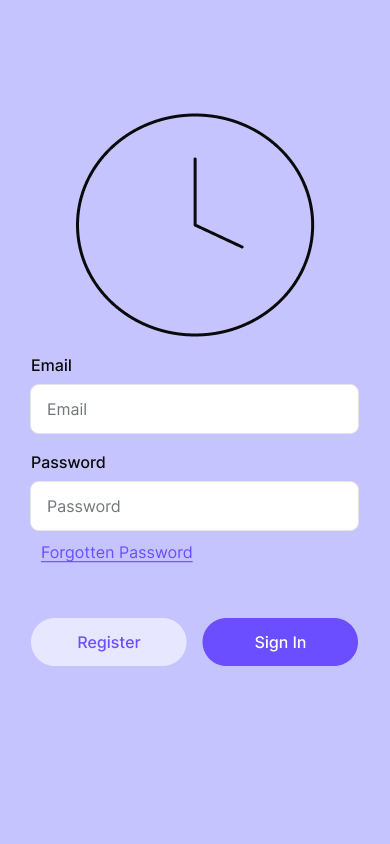
\includegraphics[width=\textwidth]{designSignIN.png}}
        \caption{Sign In}
    \end{subfigure}
    \hspace{0.5em}
    \noindent\begin{subfigure}[b]{0.23\textwidth}
        \centering
        \frame{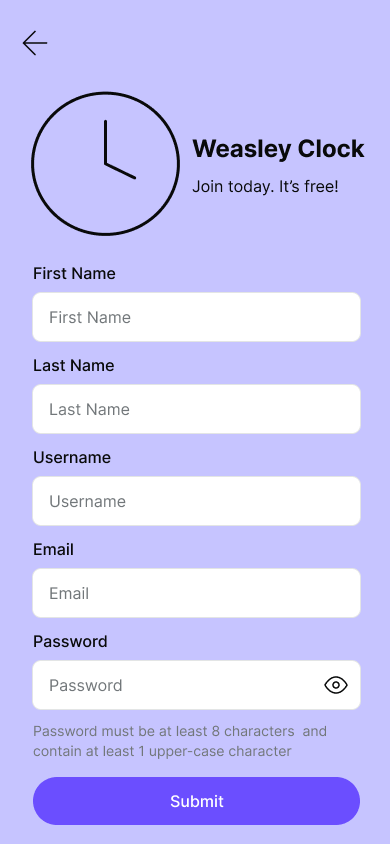
\includegraphics[width=\textwidth]{designRegister.png}}
        \caption{Register}
    \end{subfigure}
    \hspace{0.5em}
    \noindent\begin{subfigure}[b]{0.23\textwidth}
        \centering
        \frame{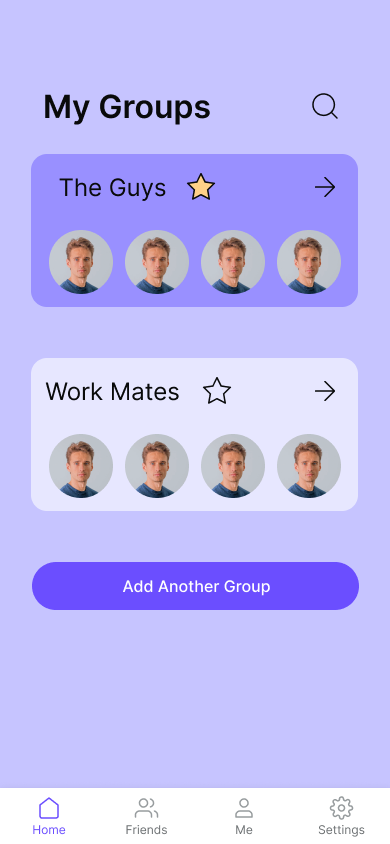
\includegraphics[width=\textwidth]{designHome.png}}
        \caption{Home}
    \end{subfigure}
    \hspace{0.5em}
    \noindent\begin{subfigure}[b]{0.23\textwidth}
        \centering
        \frame{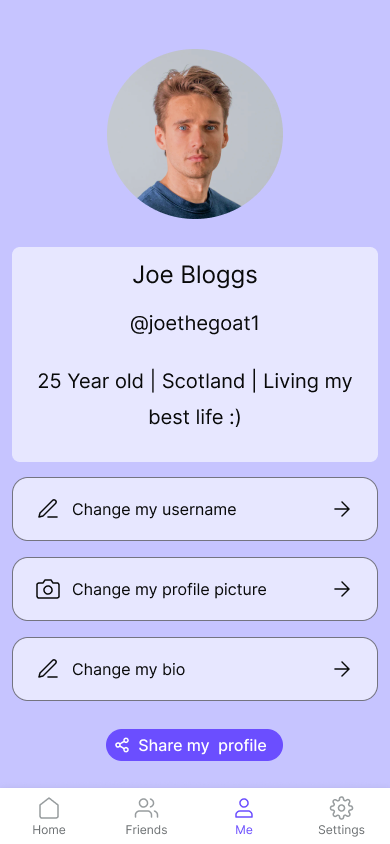
\includegraphics[width=\textwidth]{designProfile.png}}
        \caption{User Profile}
    \end{subfigure}
    \vskip\baselineskip
    \noindent\begin{subfigure}[b]{0.23\textwidth}
        \centering
        \frame{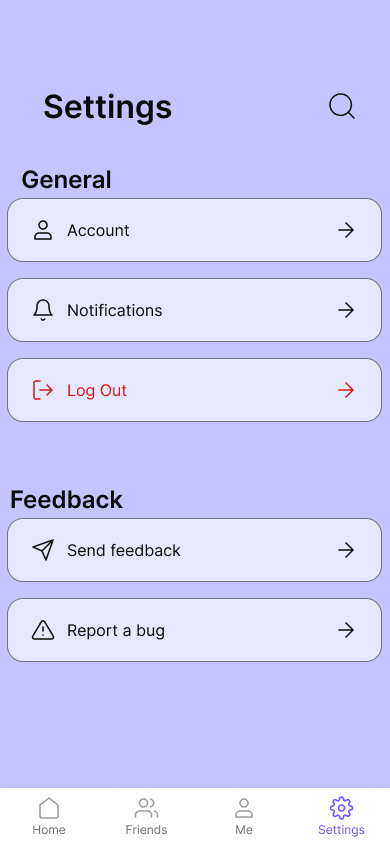
\includegraphics[width=\textwidth]{designSettings.png}}
        \caption{Settings}
    \end{subfigure}
    \hspace{0.5em}
    \noindent\begin{subfigure}[b]{0.23\textwidth}
        \centering
        \frame{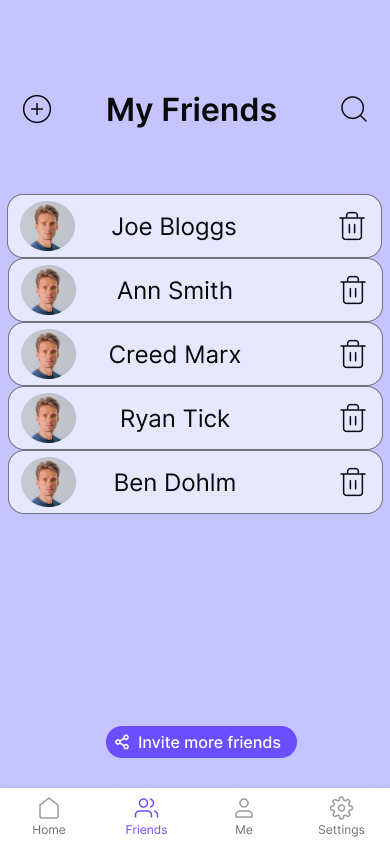
\includegraphics[width=\textwidth]{designFriends.png}}
        \caption{Friends}
    \end{subfigure}
    \hspace{0.5em}
    \noindent\begin{subfigure}[b]{0.23\textwidth}
        \centering
        \frame{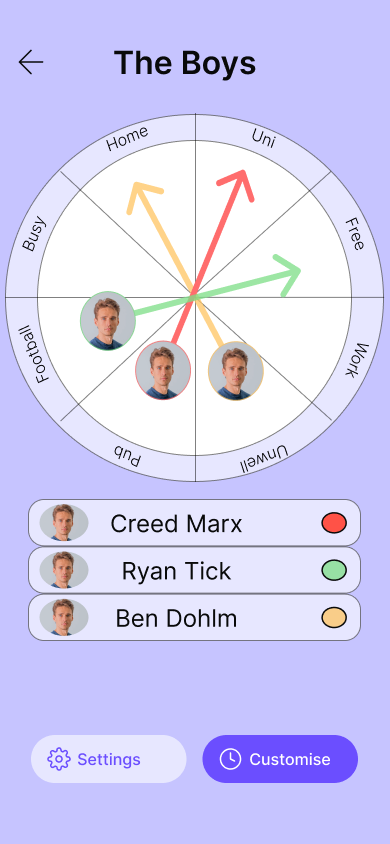
\includegraphics[width=\textwidth]{designClock.png}}
        \caption{Group}
    \end{subfigure}
    \hspace{0.5em}
    \noindent\begin{subfigure}[b]{0.23\textwidth}
        \centering
        \frame{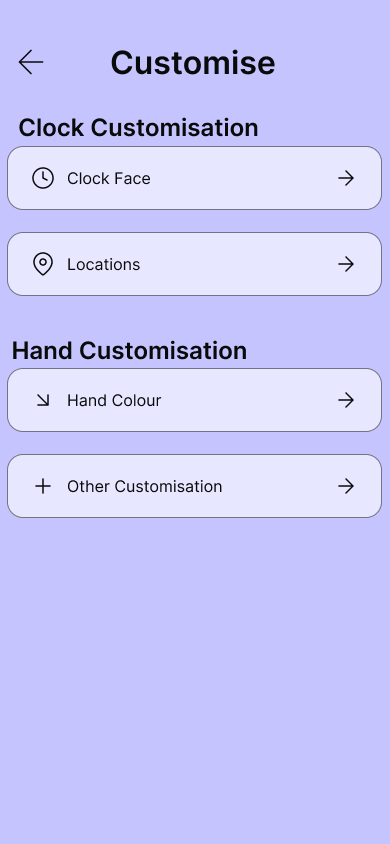
\includegraphics[width=\textwidth]{designGroupCust.png}}
        \caption{Group Customisation}
    \end{subfigure}
    \end{figure}
    \begin{figure}
    \ContinuedFloat
    \centering
    \noindent\begin{subfigure}[b]{0.23\textwidth}
        \centering
        \frame{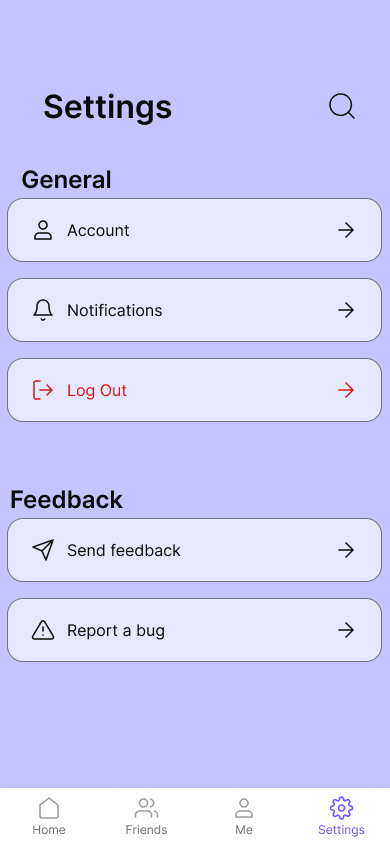
\includegraphics[width=\textwidth]{designGroupSett.png}}
        \caption{Group Settings}
    \end{subfigure}
    \hspace{0.5em}
    \noindent\begin{subfigure}[b]{0.23\textwidth}
        \centering
        \frame{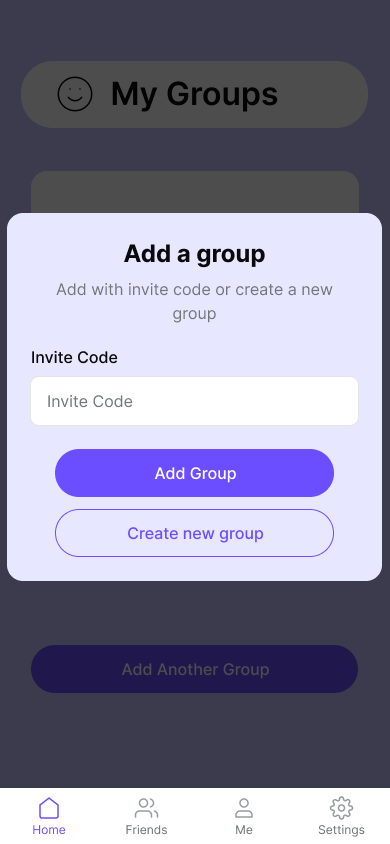
\includegraphics[width=\textwidth]{designAddGroup.png}}
        \caption{Add Group}
    \end{subfigure}
    \hspace{0.5em}
    \noindent\begin{subfigure}[b]{0.23\textwidth}
        \centering
        \frame{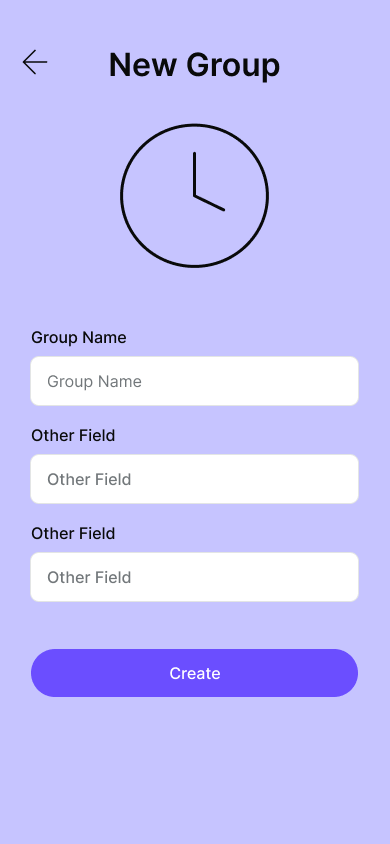
\includegraphics[width=\textwidth]{designNewGroup.png}}
        \caption{New Group }
    \end{subfigure}
    \hspace{0.5em}
    \noindent\begin{subfigure}[b]{0.23\textwidth}
        \centering
        \frame{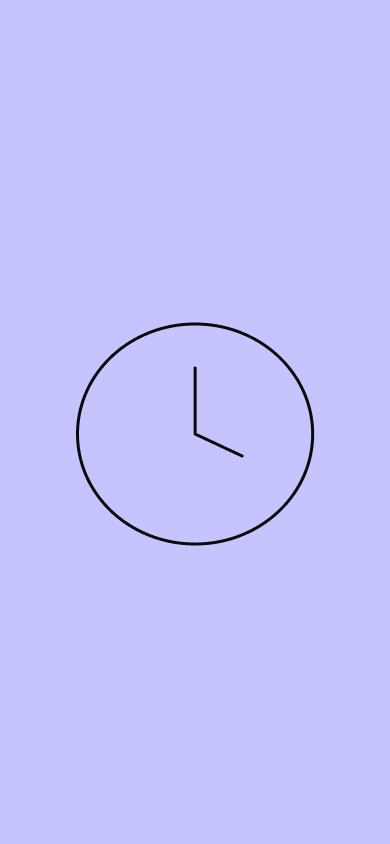
\includegraphics[width=\textwidth]{splash.png}}
        \caption{Splash}\label{splash}
    \end{subfigure}
    \caption{Figma Designs}
\end{figure}
\FloatBarrier


\section{Application User Interface}\label{appendix:appScreens}
\begin{figure}[!htbp]
    \centering
    \noindent\begin{subfigure}[b]{0.23\textwidth}
        \centering
        \frame{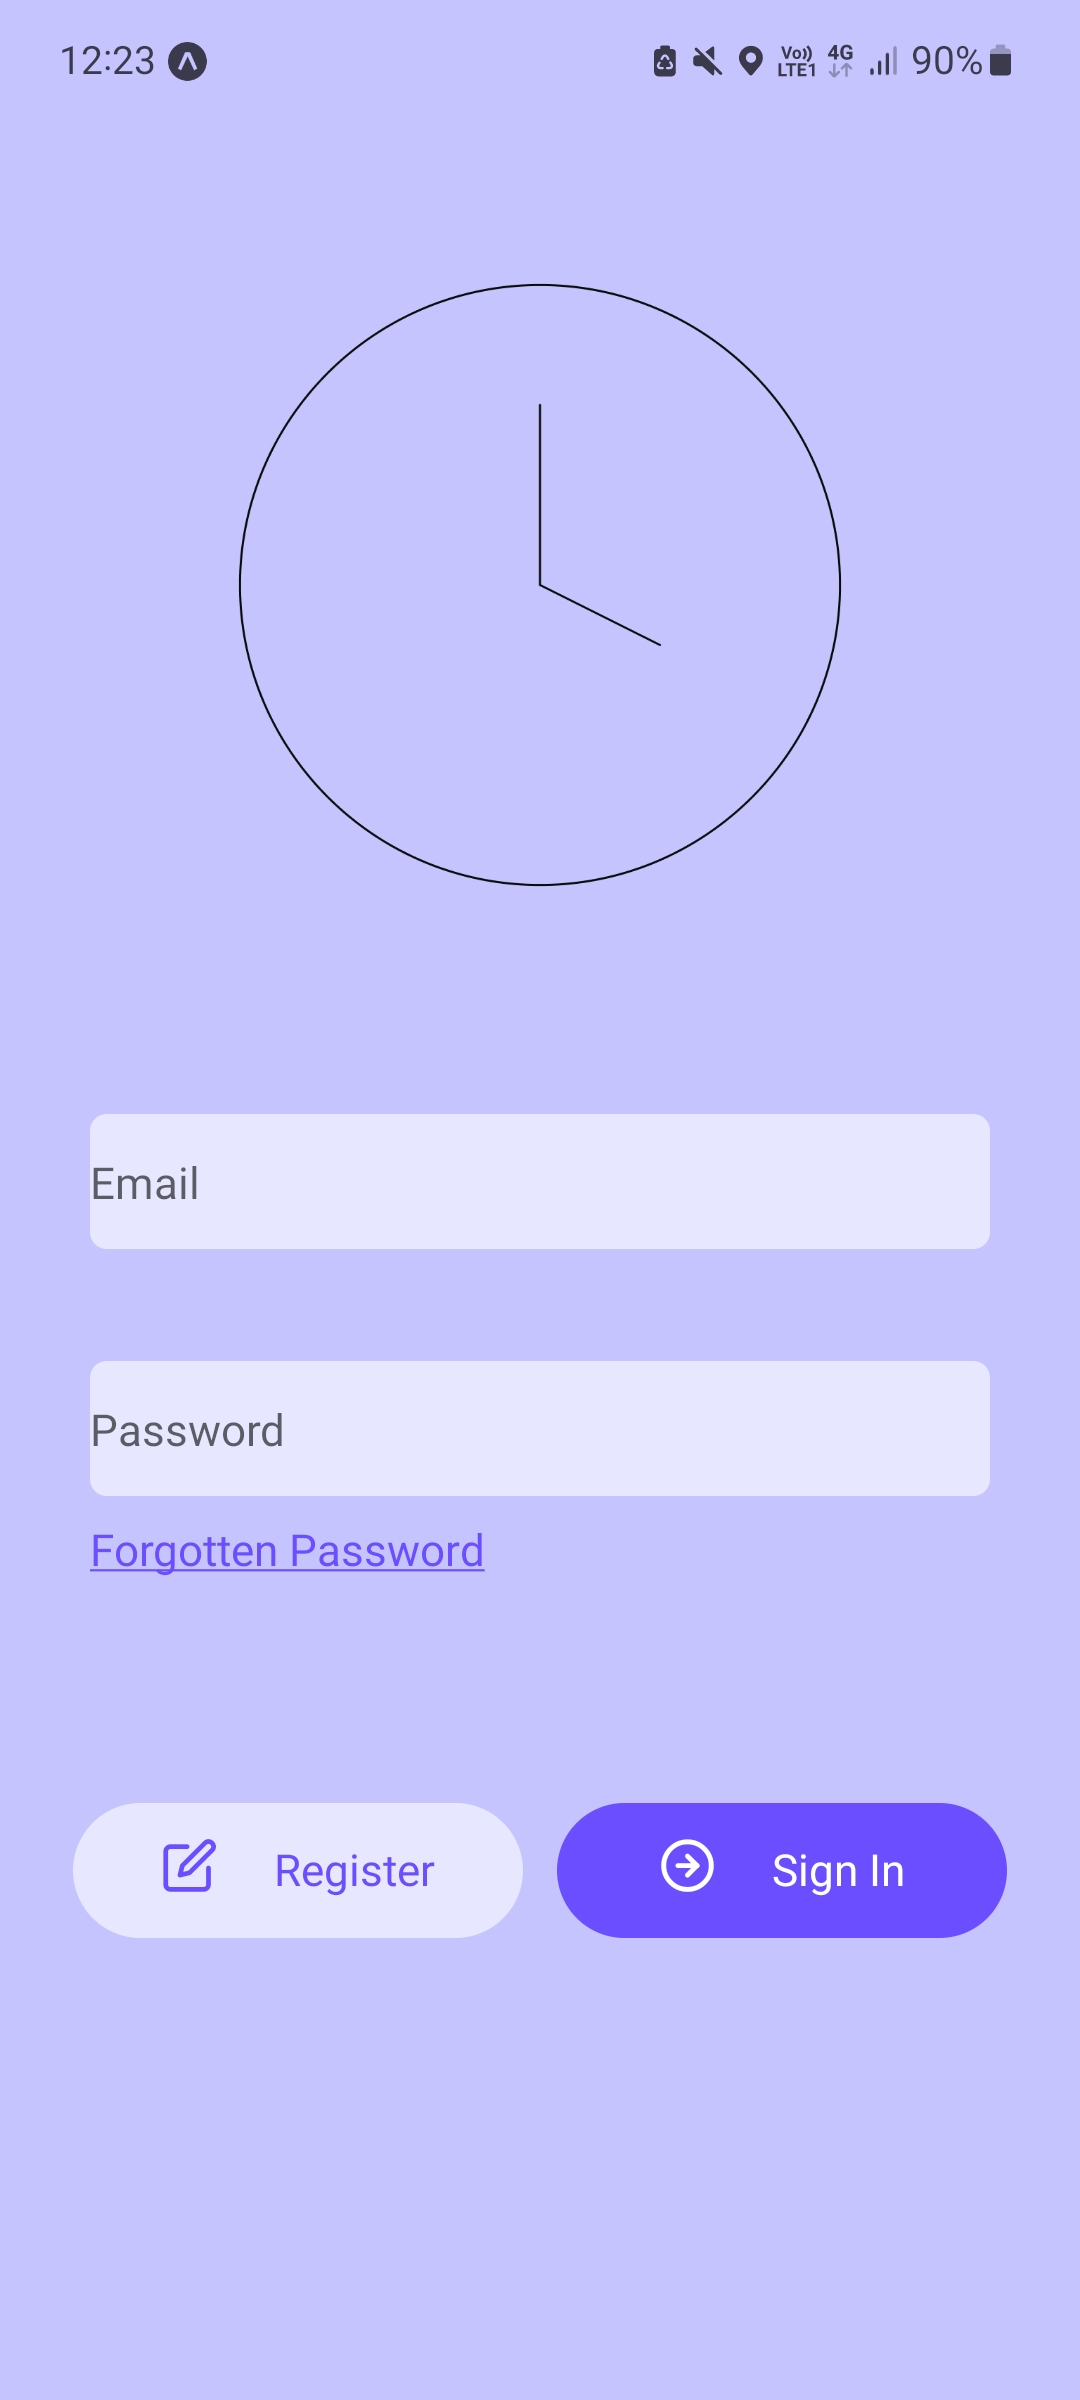
\includegraphics[width=\textwidth]{signIn.jpg}}
        \caption{Sign In}
    \end{subfigure}
    \hspace{0.5em}
    \noindent\begin{subfigure}[b]{0.23\textwidth}
        \centering
        \frame{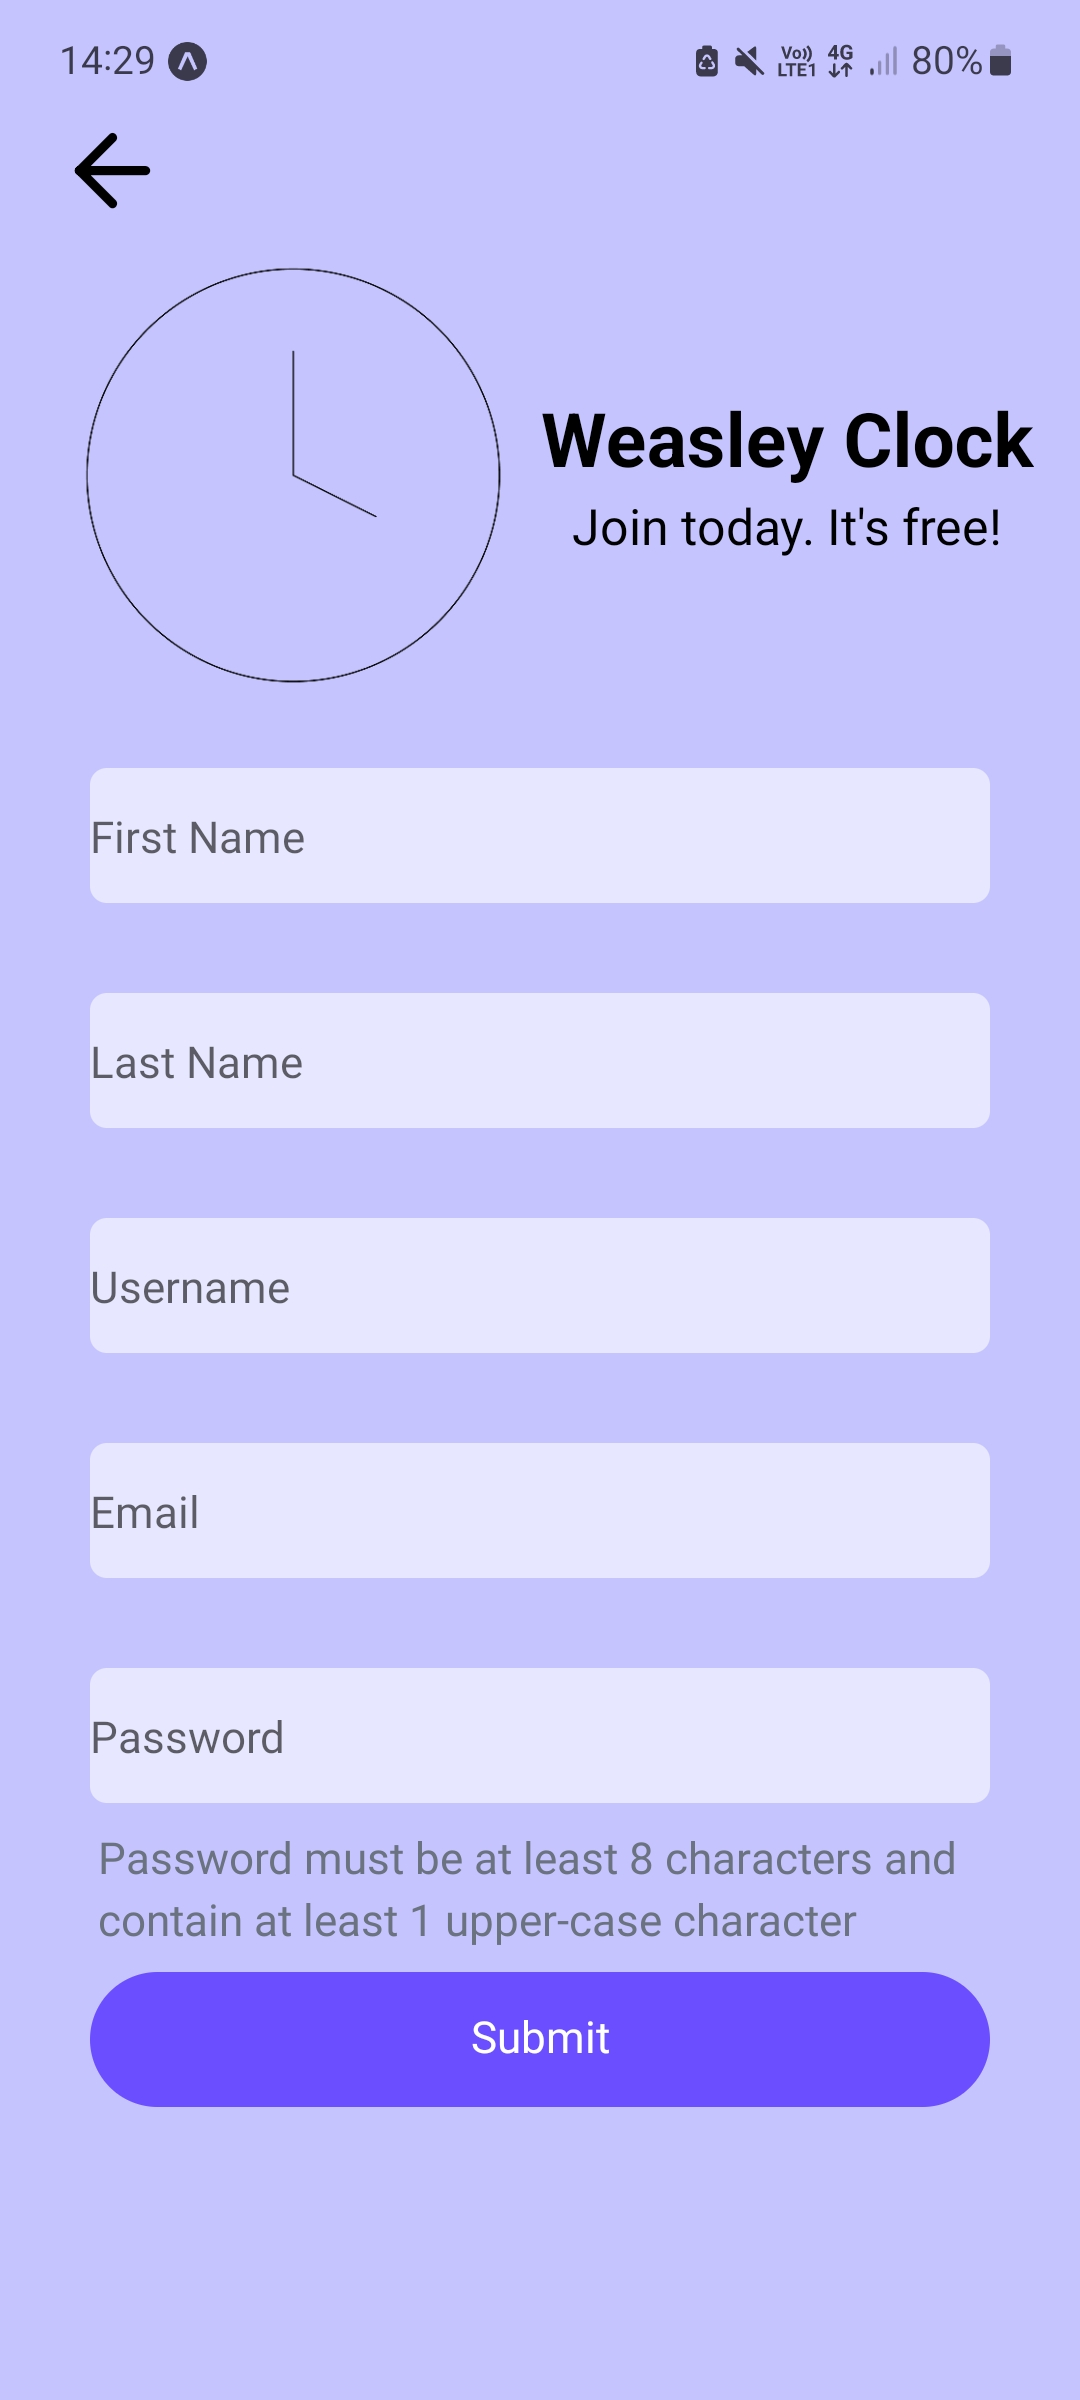
\includegraphics[width=\textwidth]{register.jpg}}
        \caption{Register}
    \end{subfigure}
    \hspace{0.5em}
    \noindent\begin{subfigure}[b]{0.23\textwidth}
        \centering
        \frame{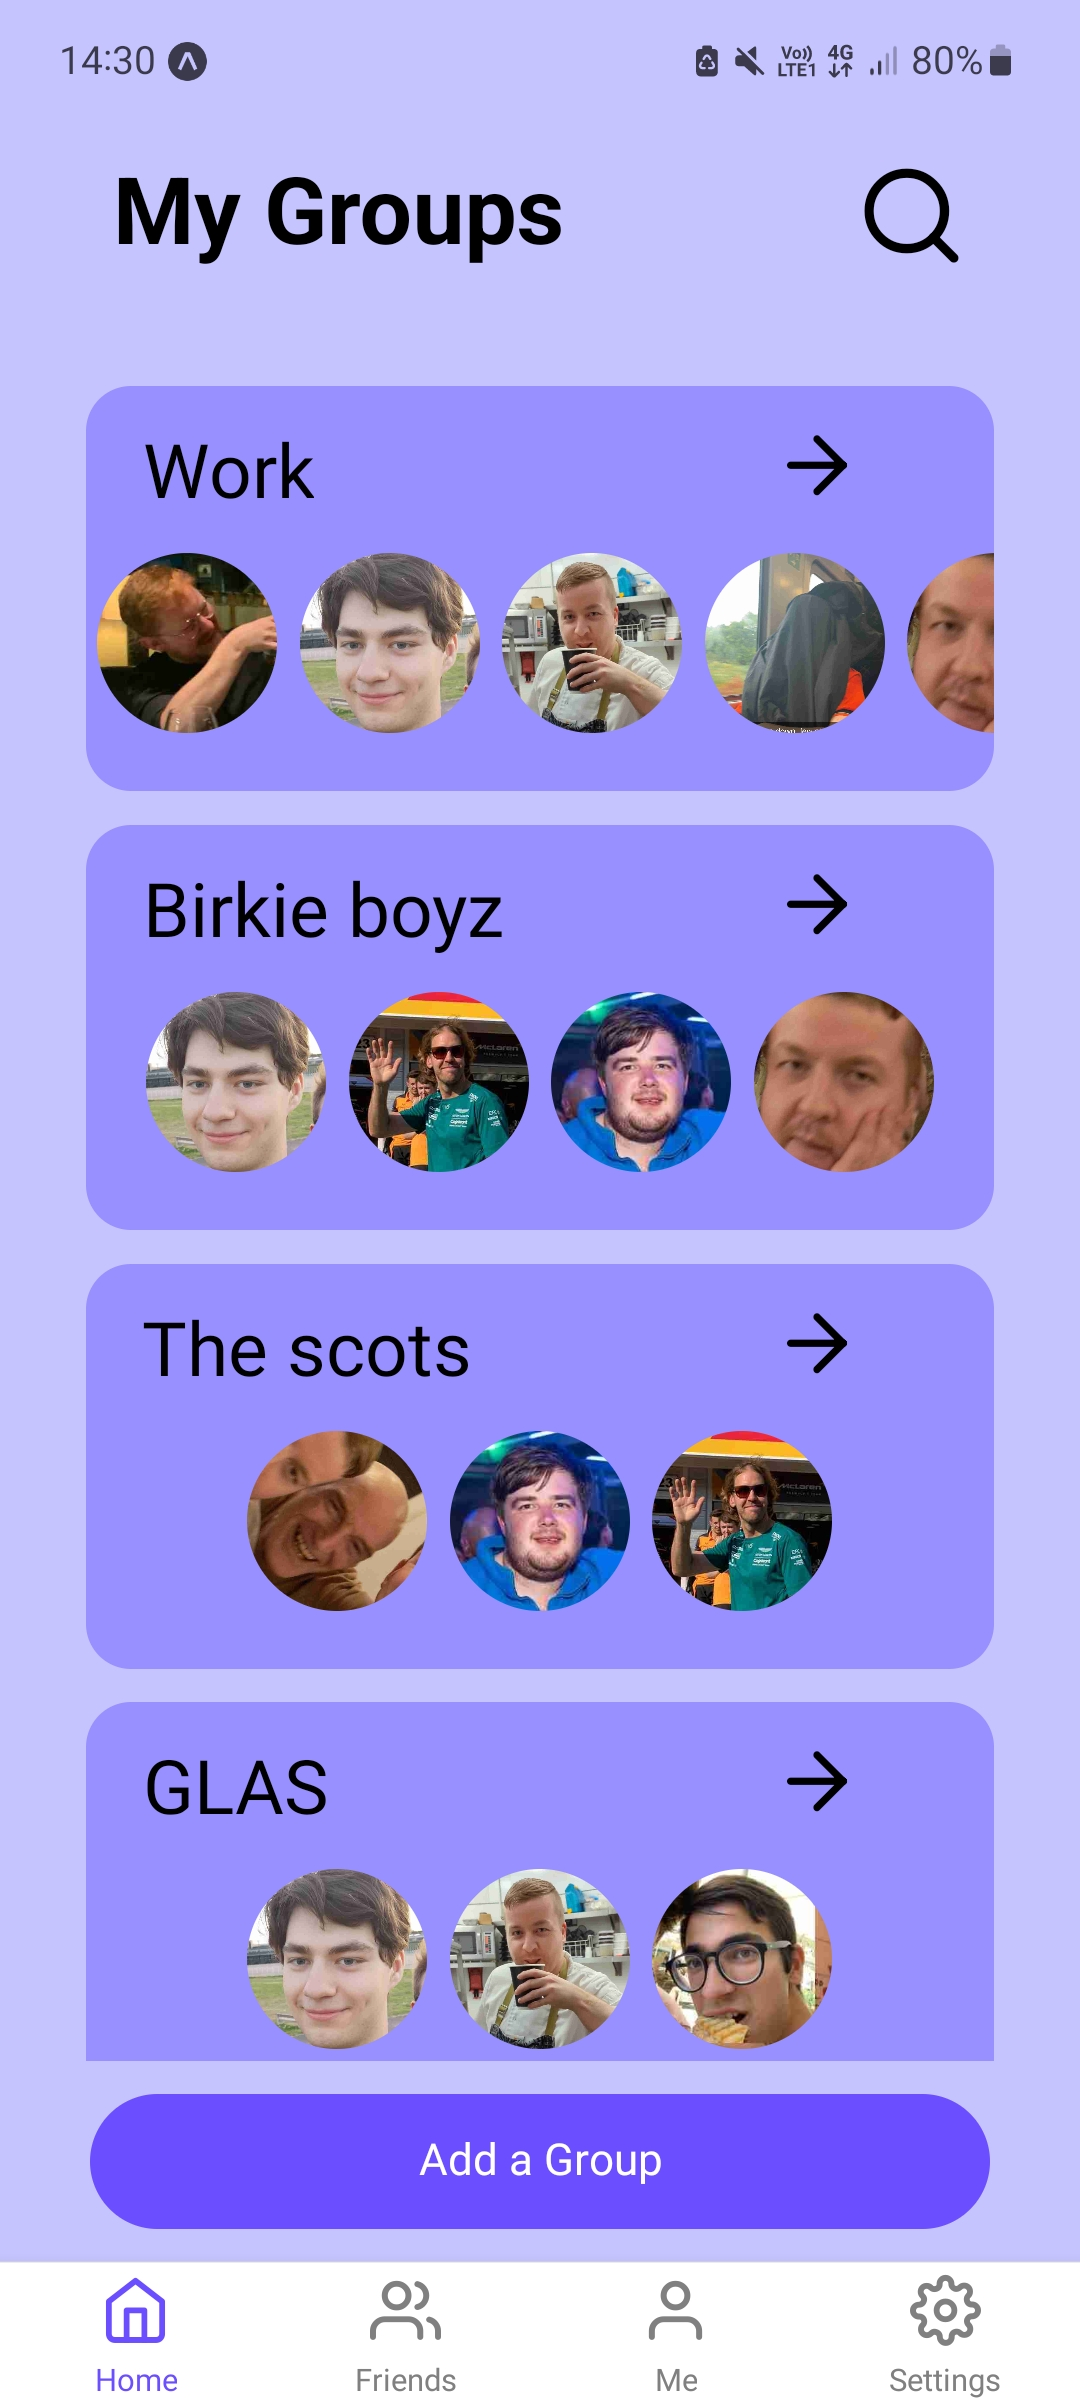
\includegraphics[width=\textwidth]{home.jpg}}
        \caption{Home}
    \end{subfigure}
    \hspace{0.5em}
    \noindent\begin{subfigure}[b]{0.23\textwidth}
        \centering
        \frame{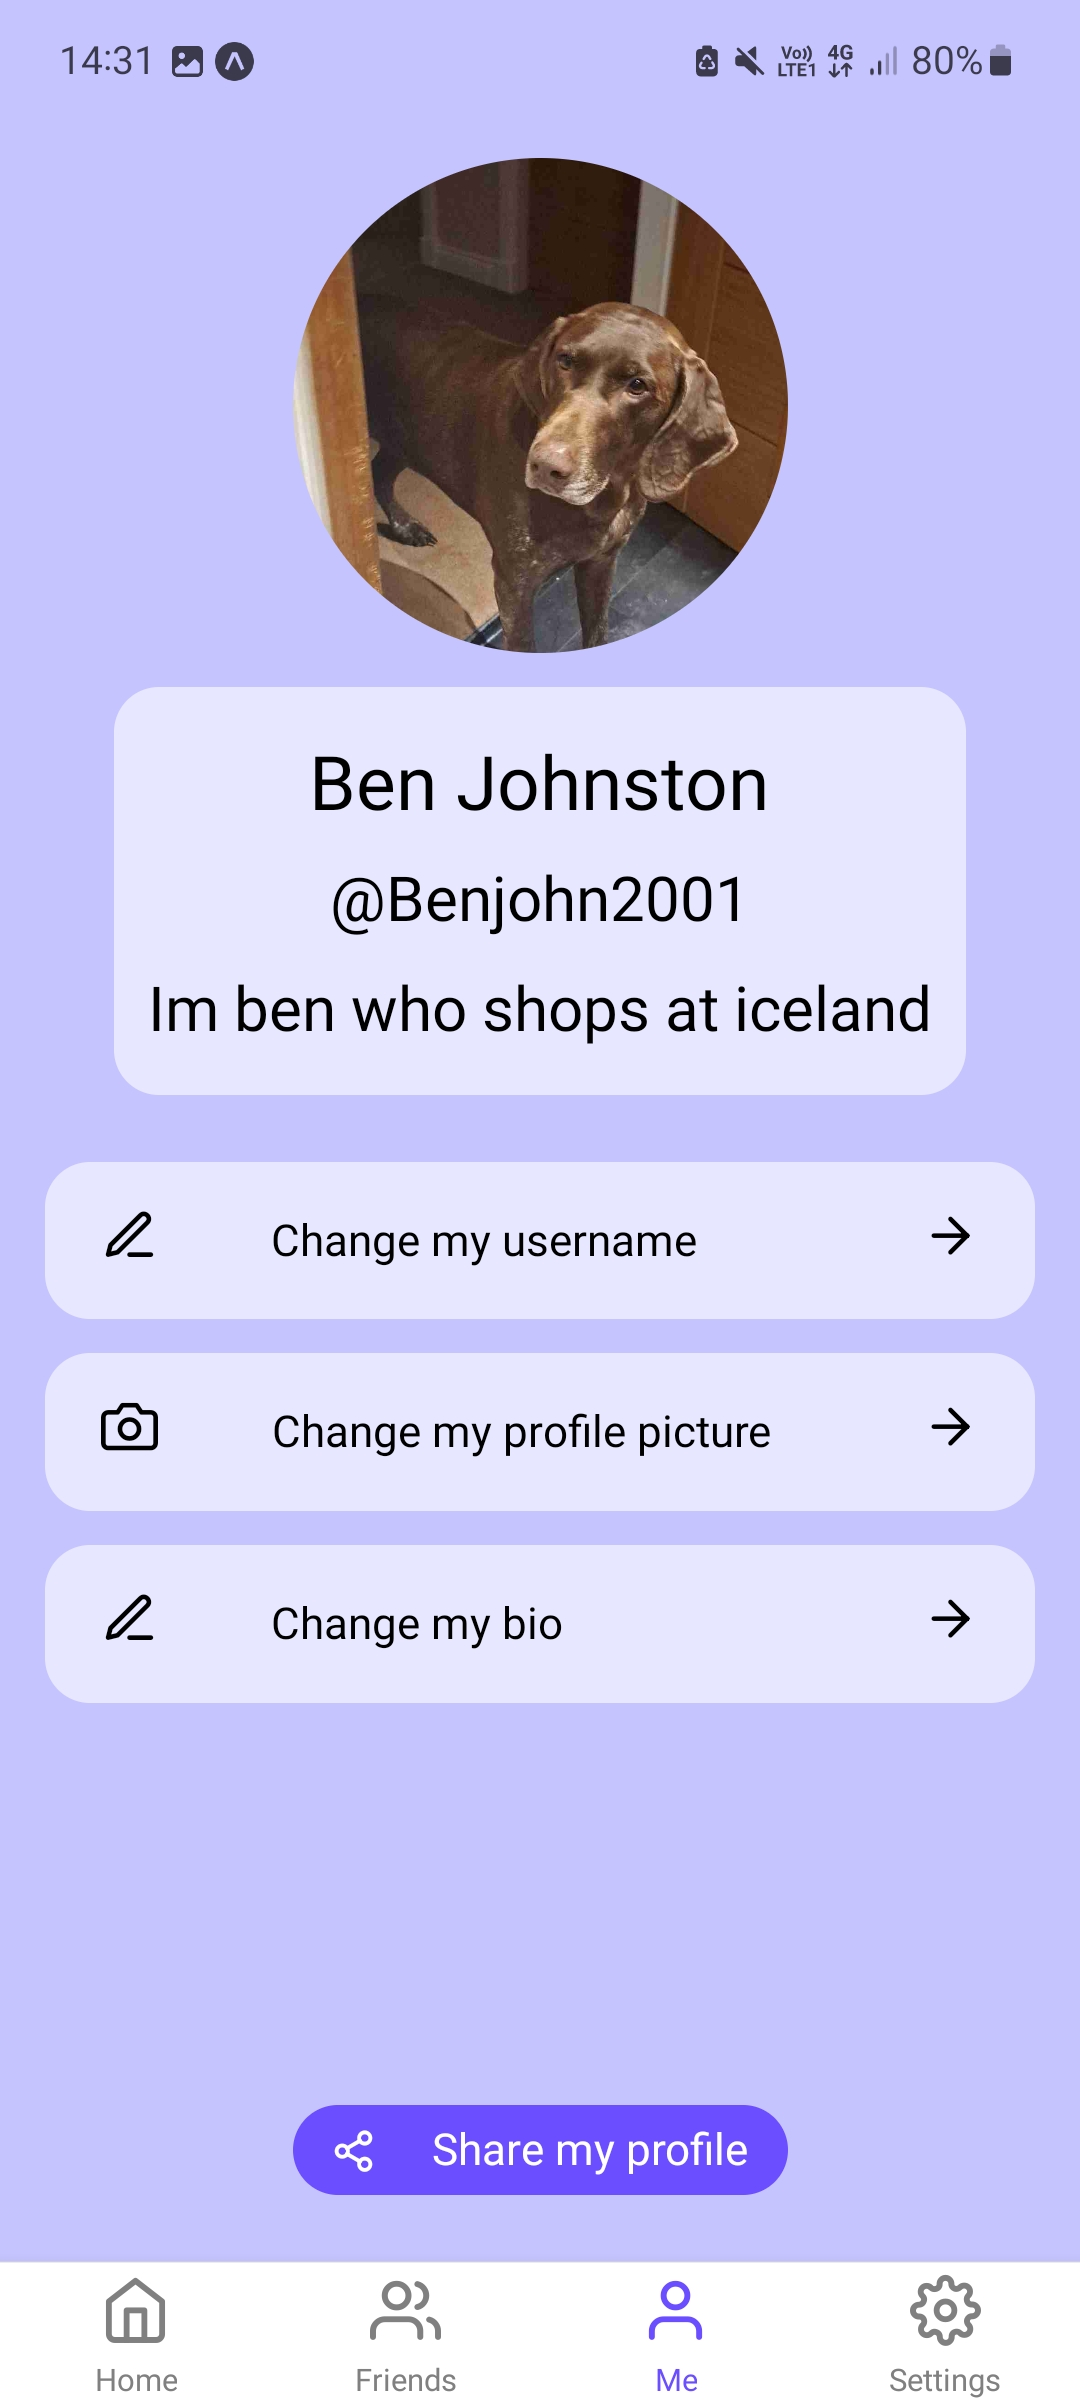
\includegraphics[width=\textwidth]{myProfile.jpg}}
        \caption{User Profile}
    \end{subfigure}
    \end{figure}
    \FloatBarrier
    \begin{figure}
    \ContinuedFloat
    \centering
    \noindent\begin{subfigure}[b]{0.23\textwidth}
        \centering
        \frame{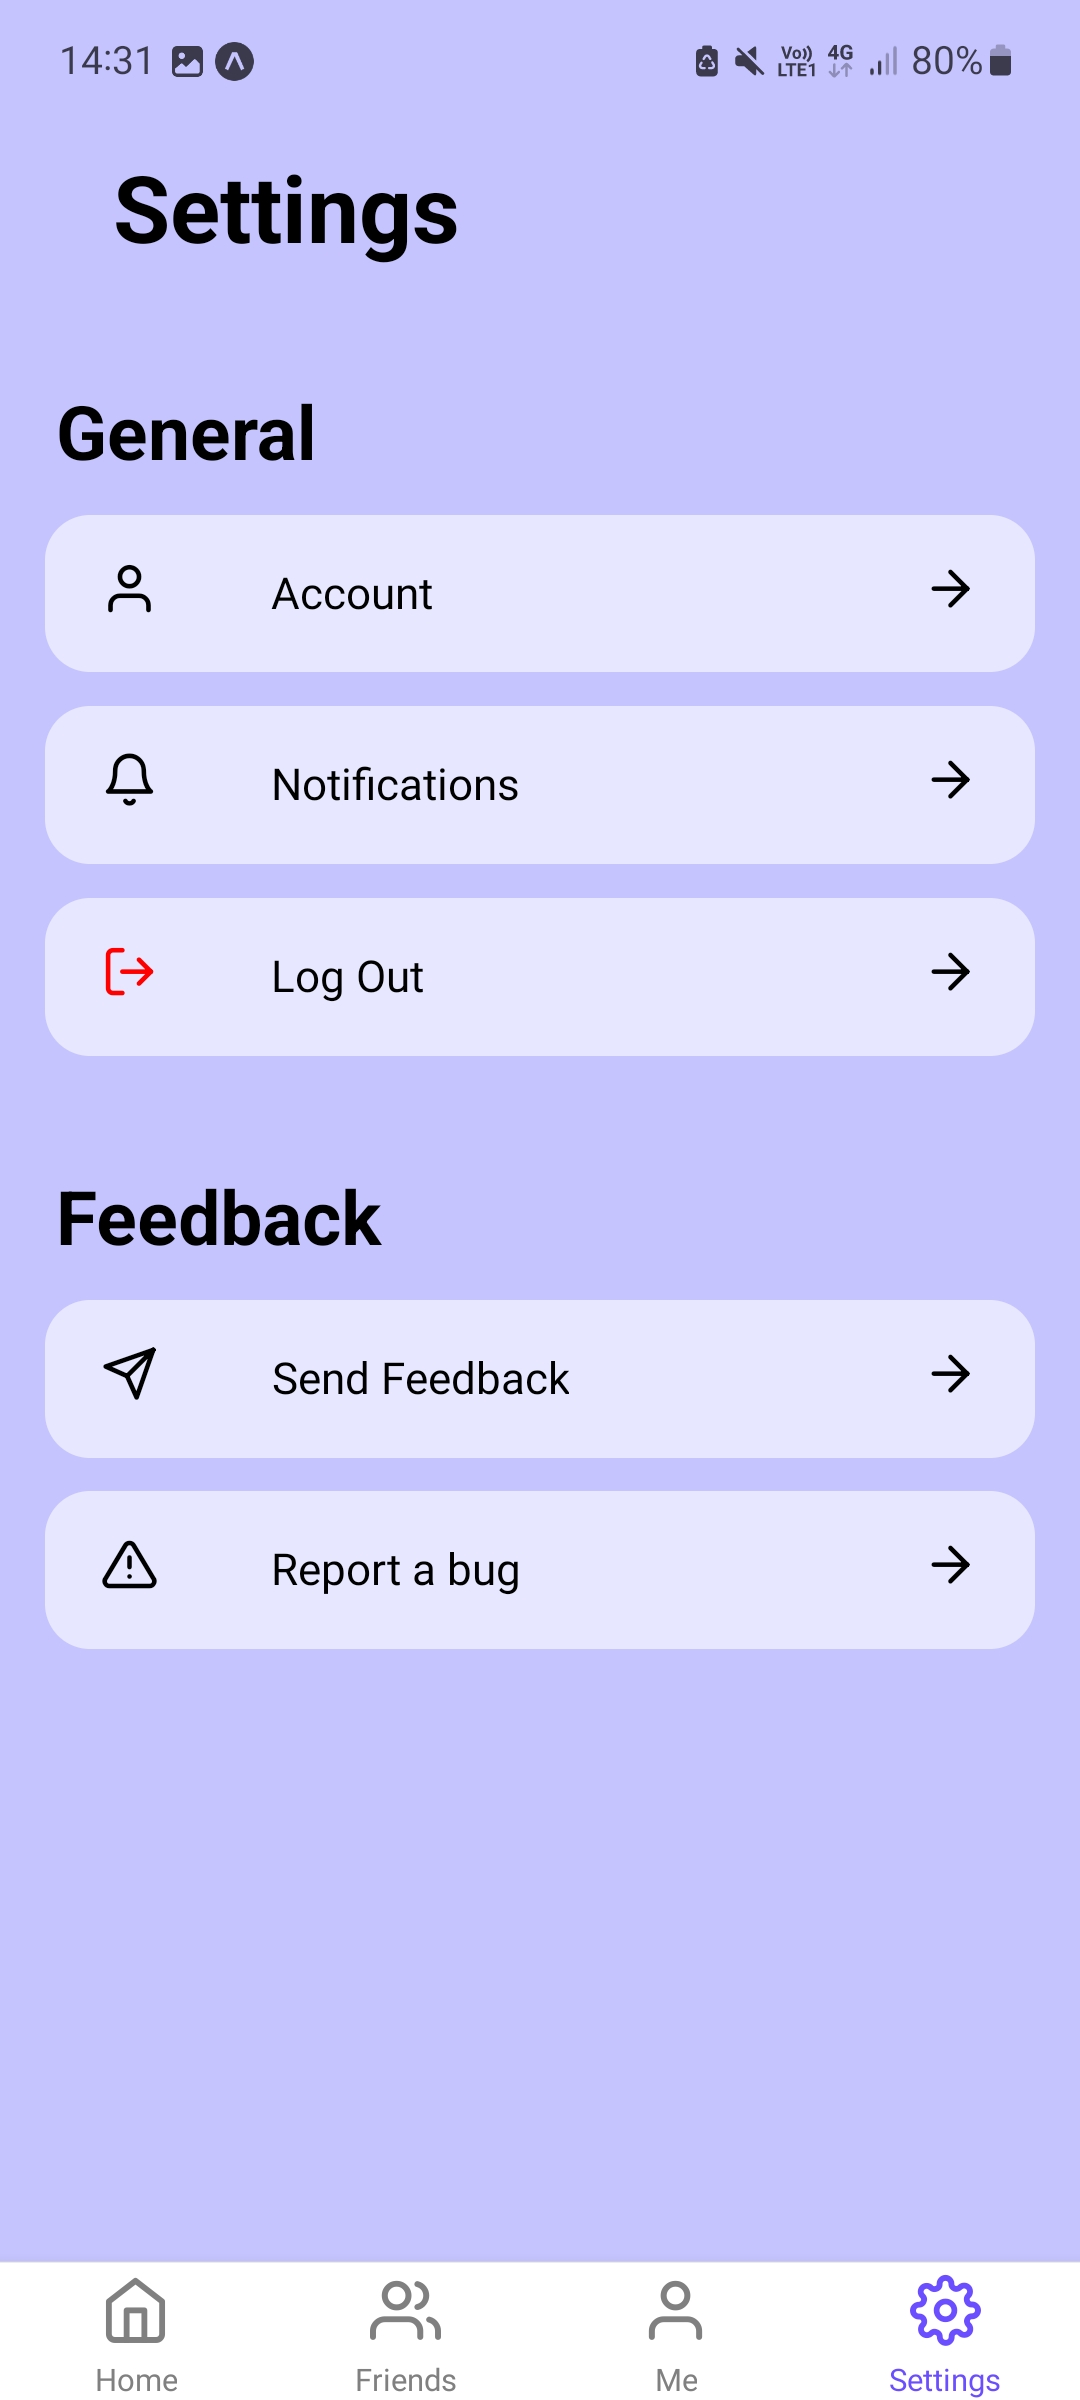
\includegraphics[width=\textwidth]{settings.jpg}}
        \caption{Settings}
    \end{subfigure}
    \hspace{0.5em}
    \noindent\begin{subfigure}[b]{0.23\textwidth}
        \centering
        \frame{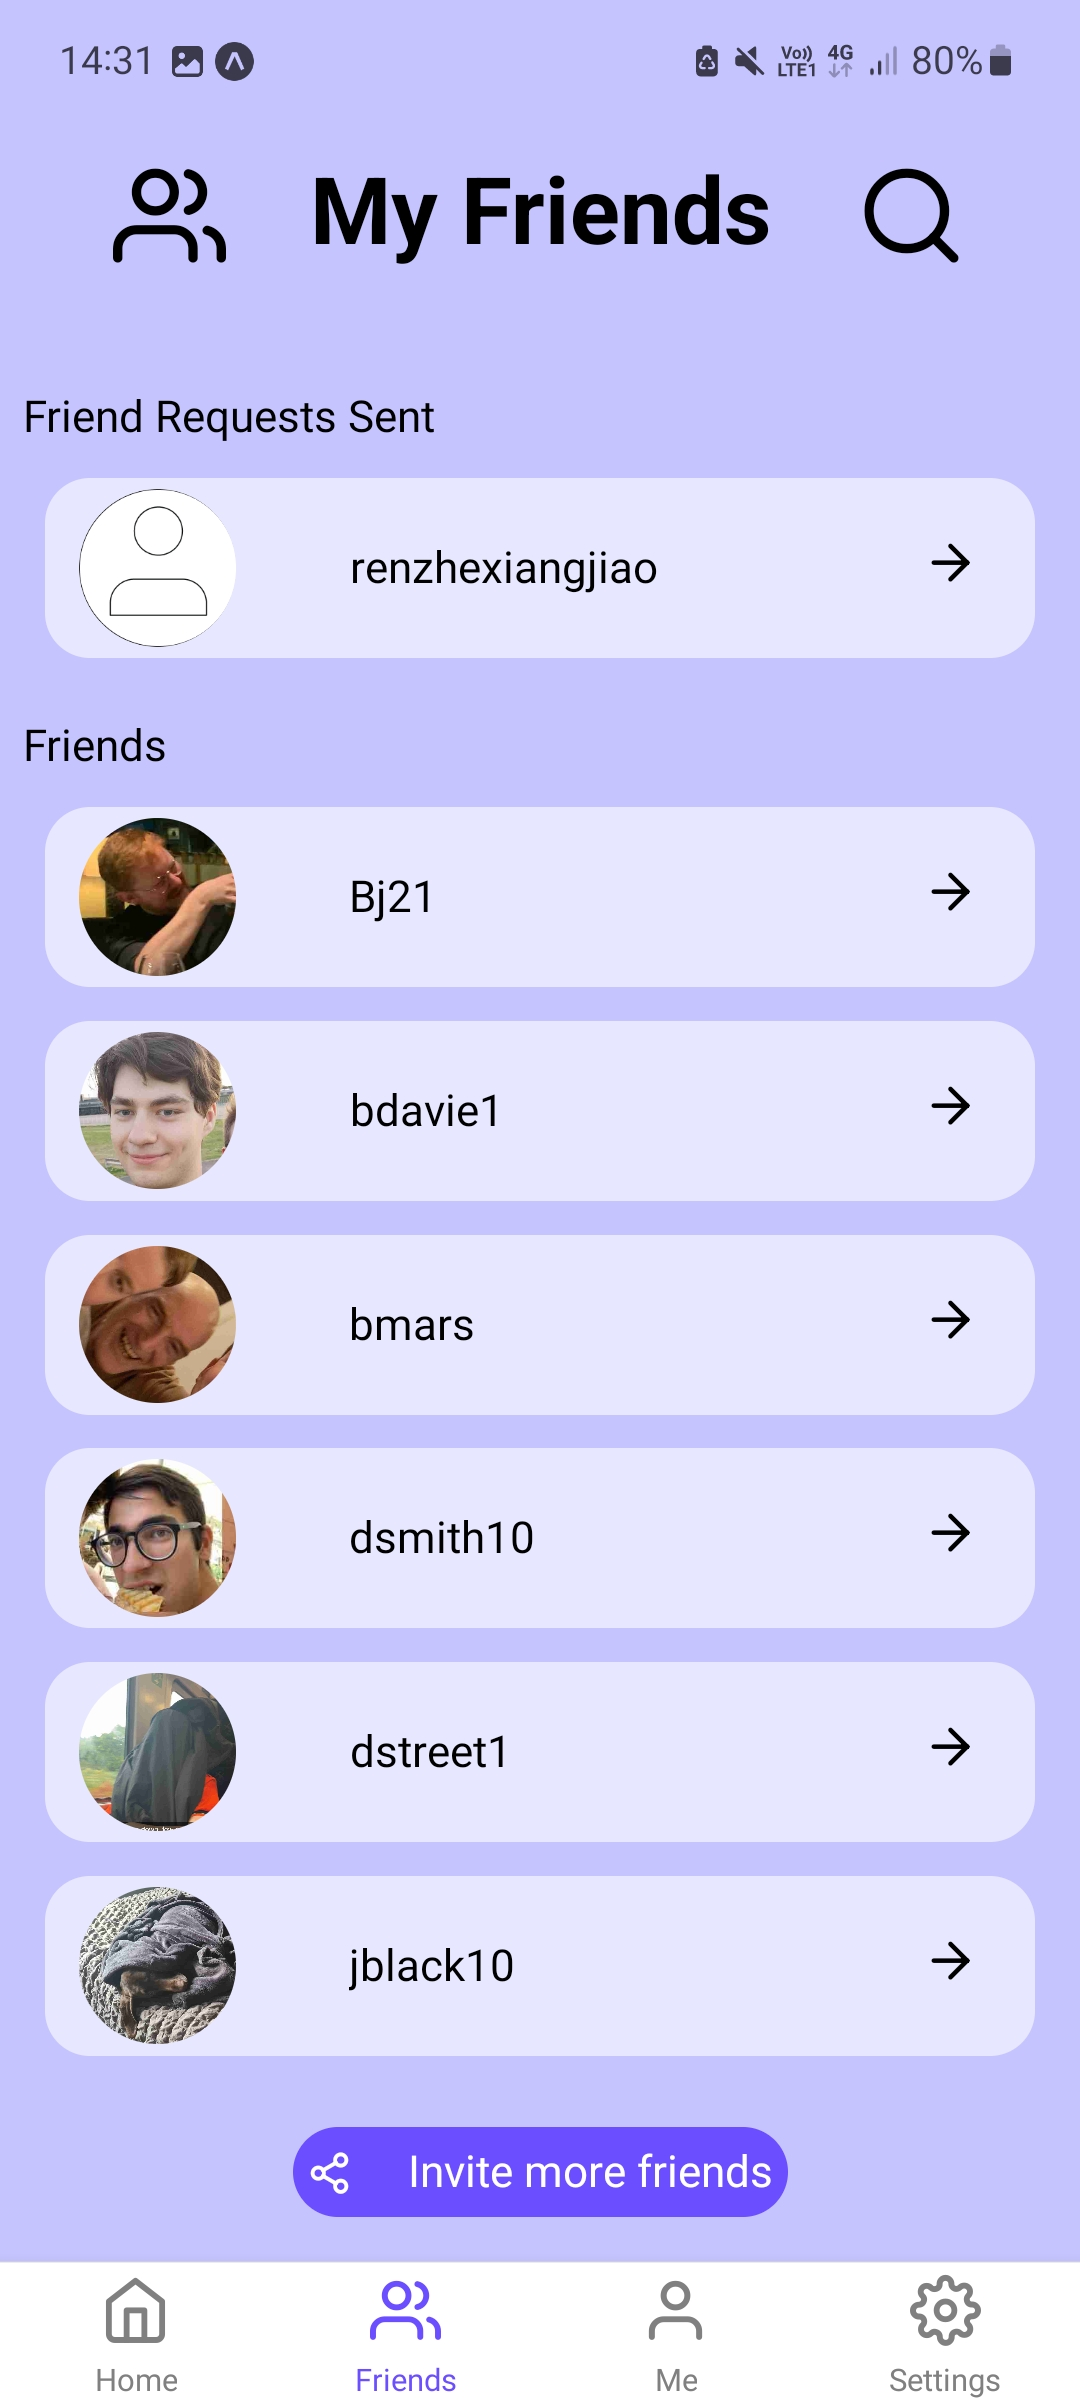
\includegraphics[width=\textwidth]{friendsList.jpg}}
        \caption{Friends List}
    \end{subfigure}
    \hspace{0.5em}
    \noindent\begin{subfigure}[b]{0.23\textwidth}
        \centering
        \frame{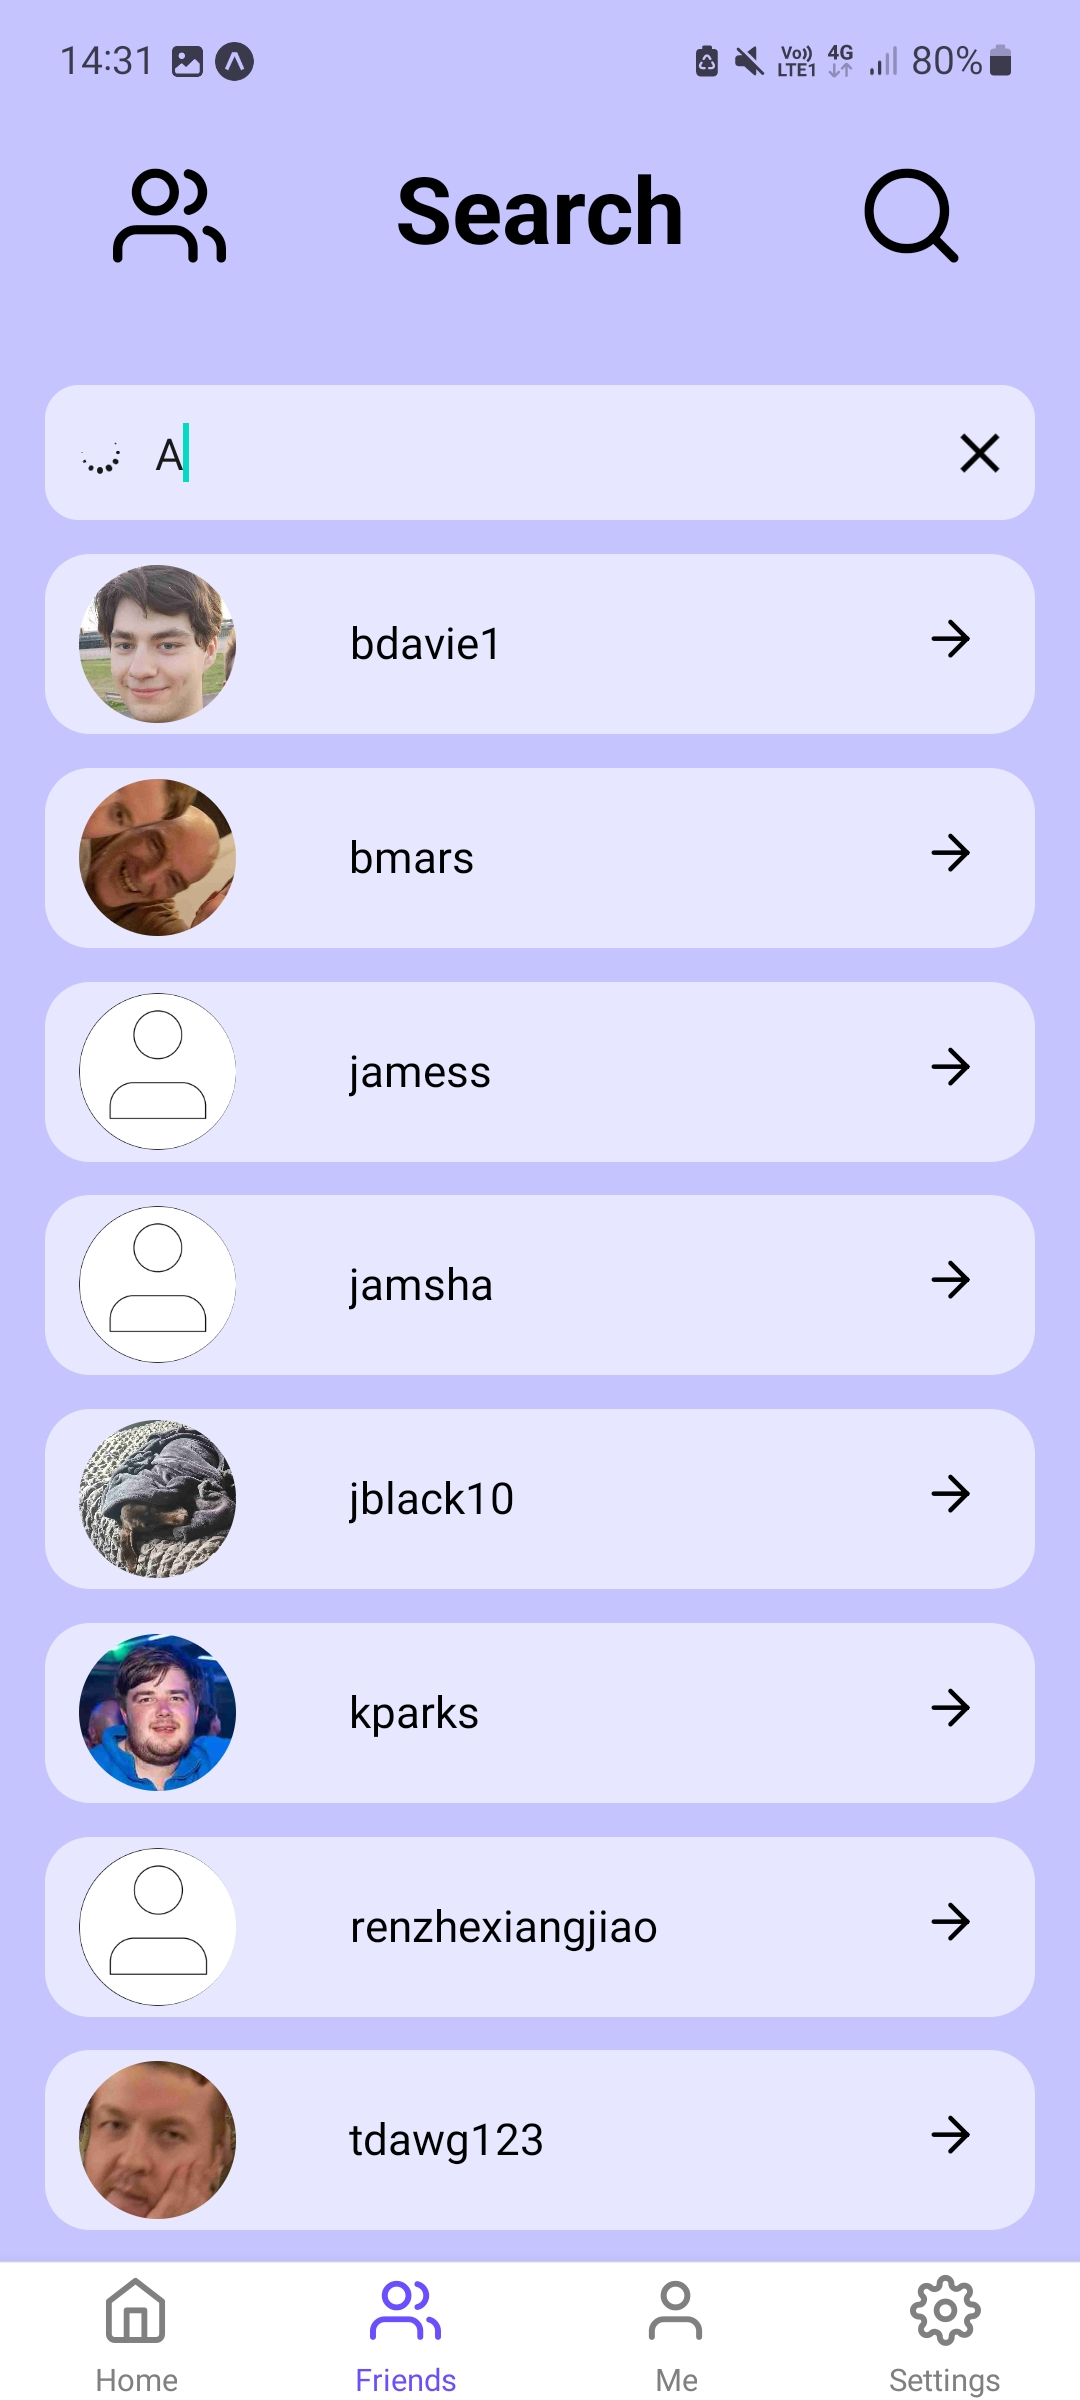
\includegraphics[width=\textwidth]{searchFriends.jpg}}
        \caption{Friends Search}
    \end{subfigure}
    \hspace{0.5em}
    \noindent\begin{subfigure}[b]{0.23\textwidth}
        \centering
        \frame{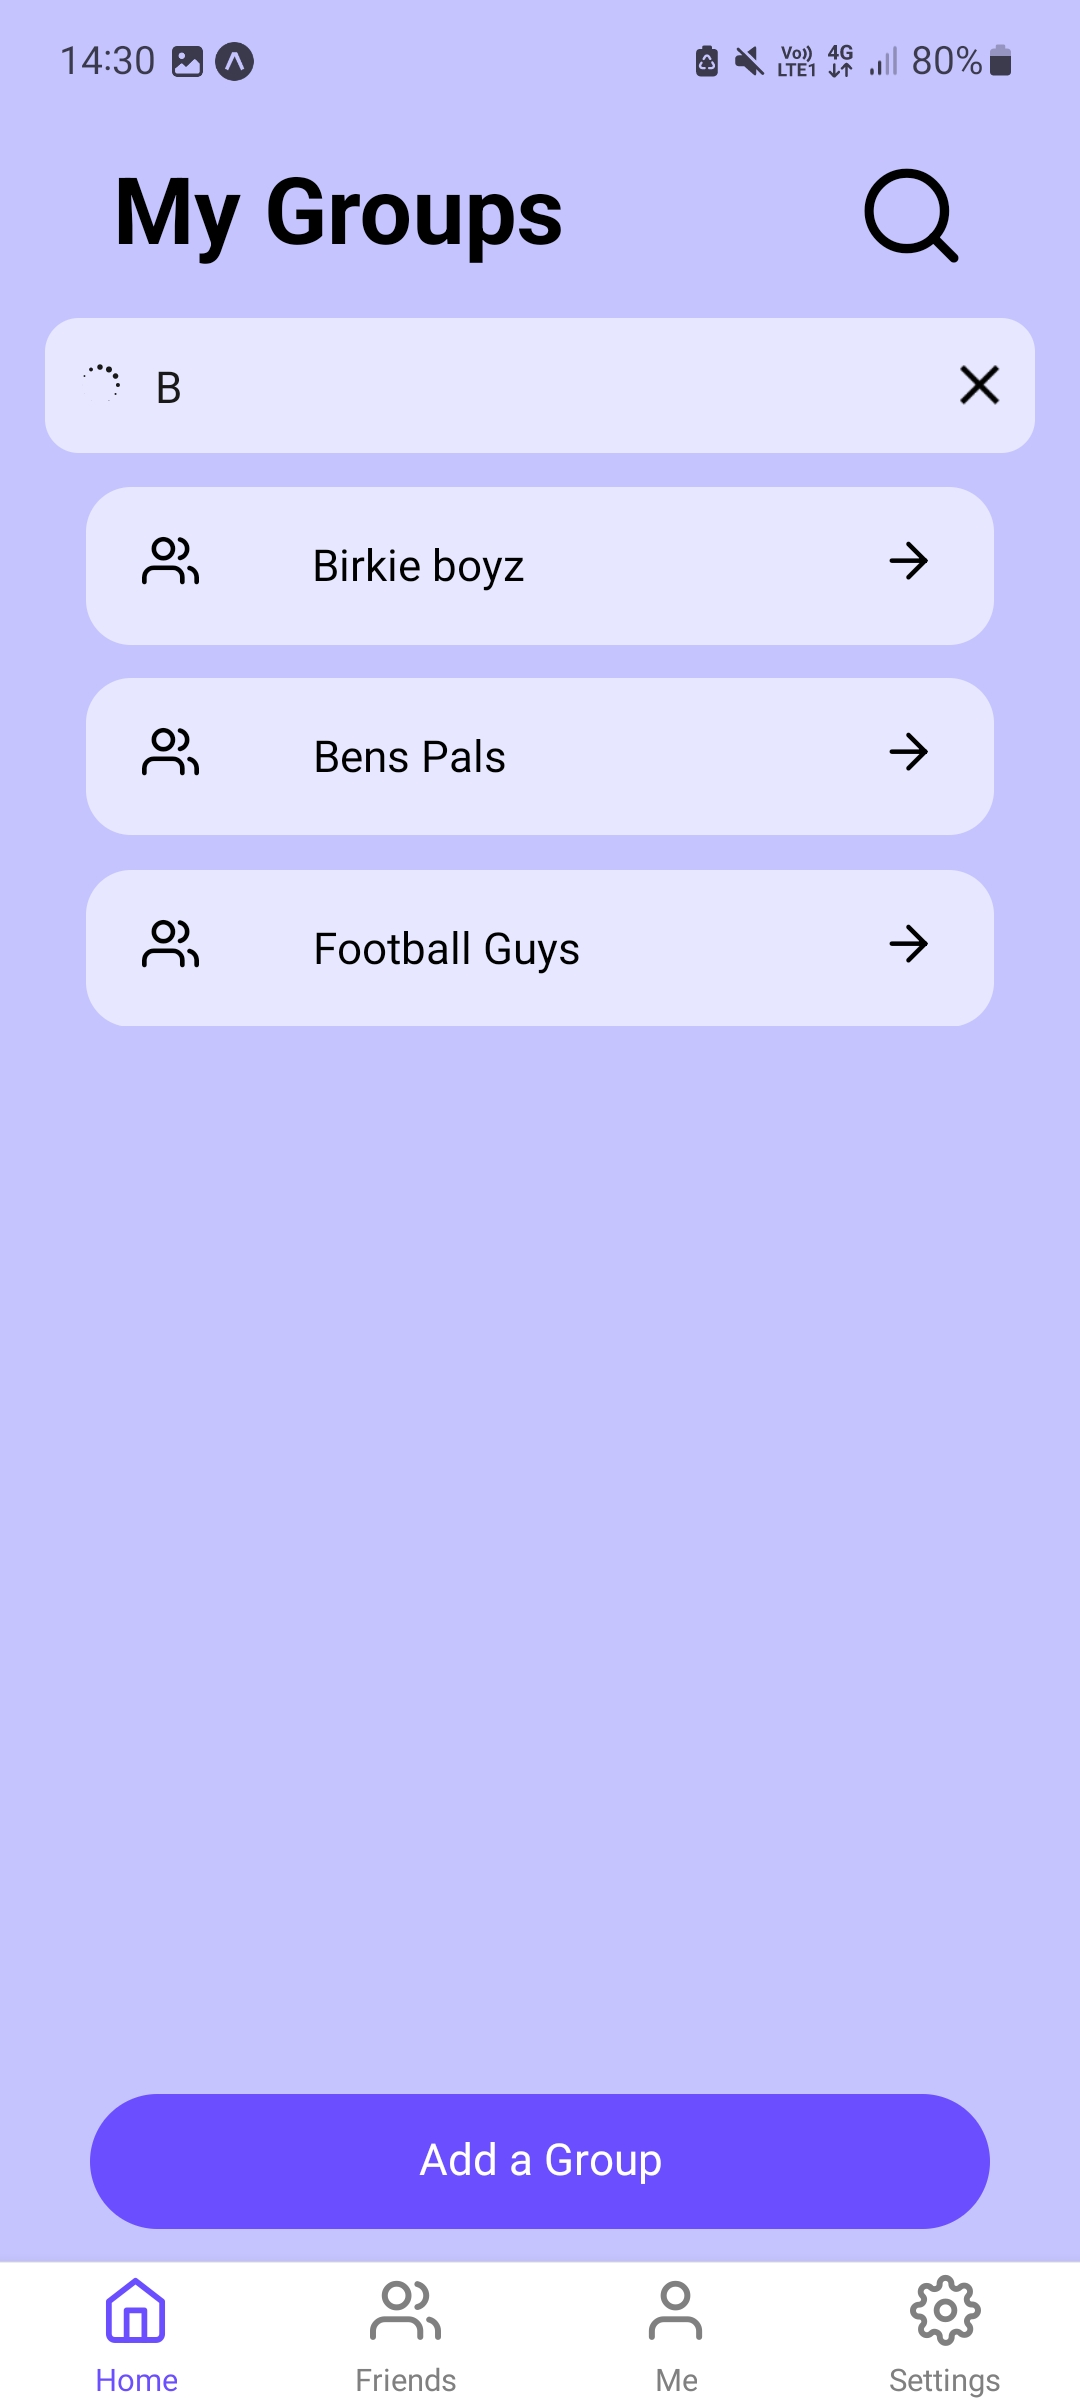
\includegraphics[width=\textwidth]{searchGroups.jpg}}
        \caption{Groups Search}
    \end{subfigure}
    \vskip\baselineskip
    \noindent\begin{subfigure}[b]{0.23\textwidth}
        \centering
        \frame{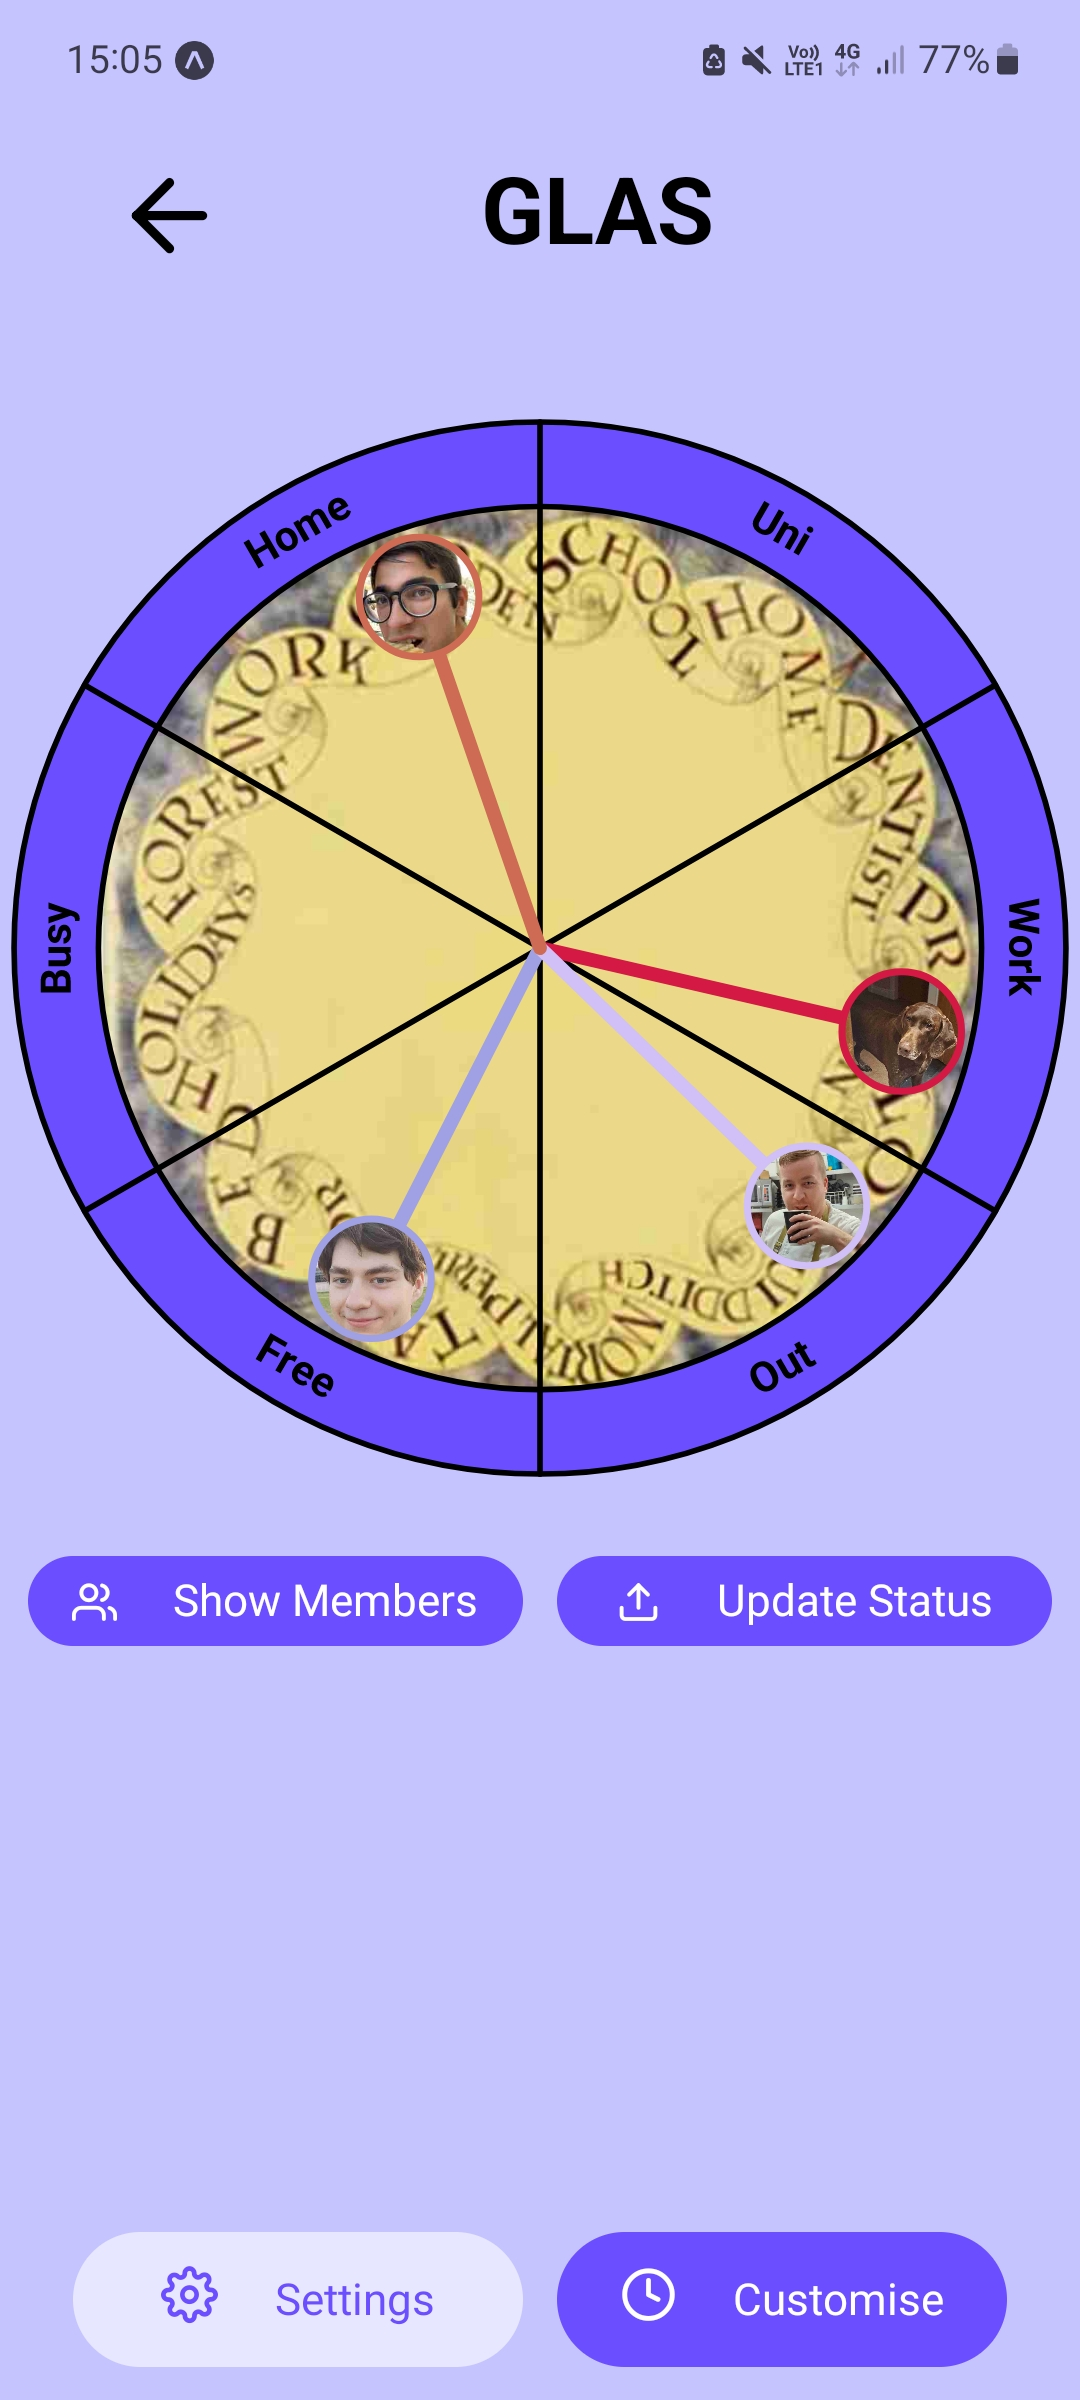
\includegraphics[width=\textwidth]{clock.jpg}}
        \caption{Group}
    \end{subfigure}
    \hspace{0.5em}
    \noindent\begin{subfigure}[b]{0.23\textwidth}
        \centering
        \frame{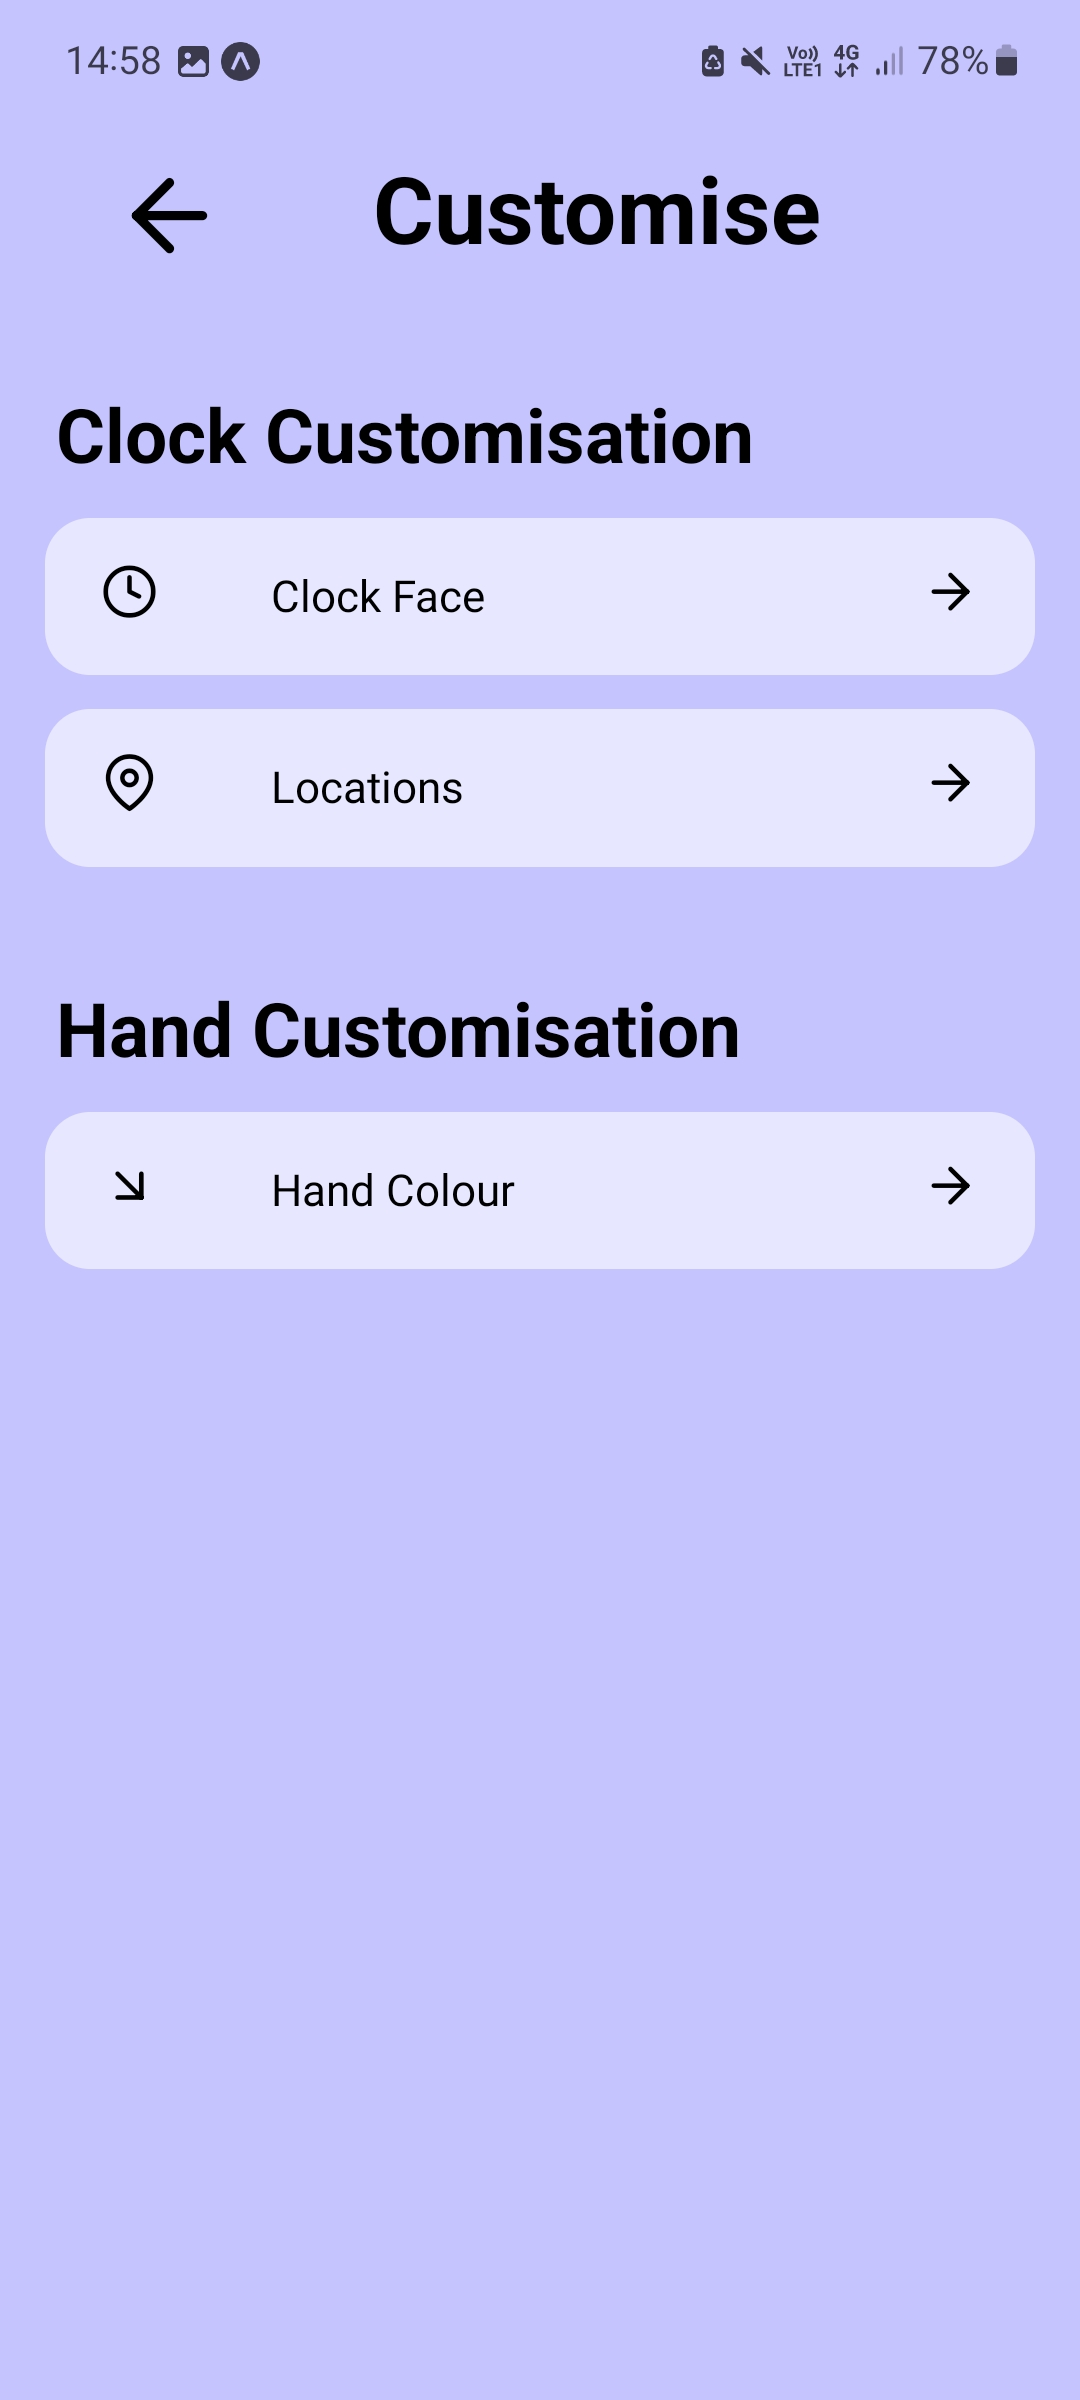
\includegraphics[width=\textwidth]{groupCustomisation.jpg}}
        \caption{Group Customisation}
    \end{subfigure}
    \hspace{0.5em}
    \noindent\begin{subfigure}[b]{0.23\textwidth}
        \centering
        \frame{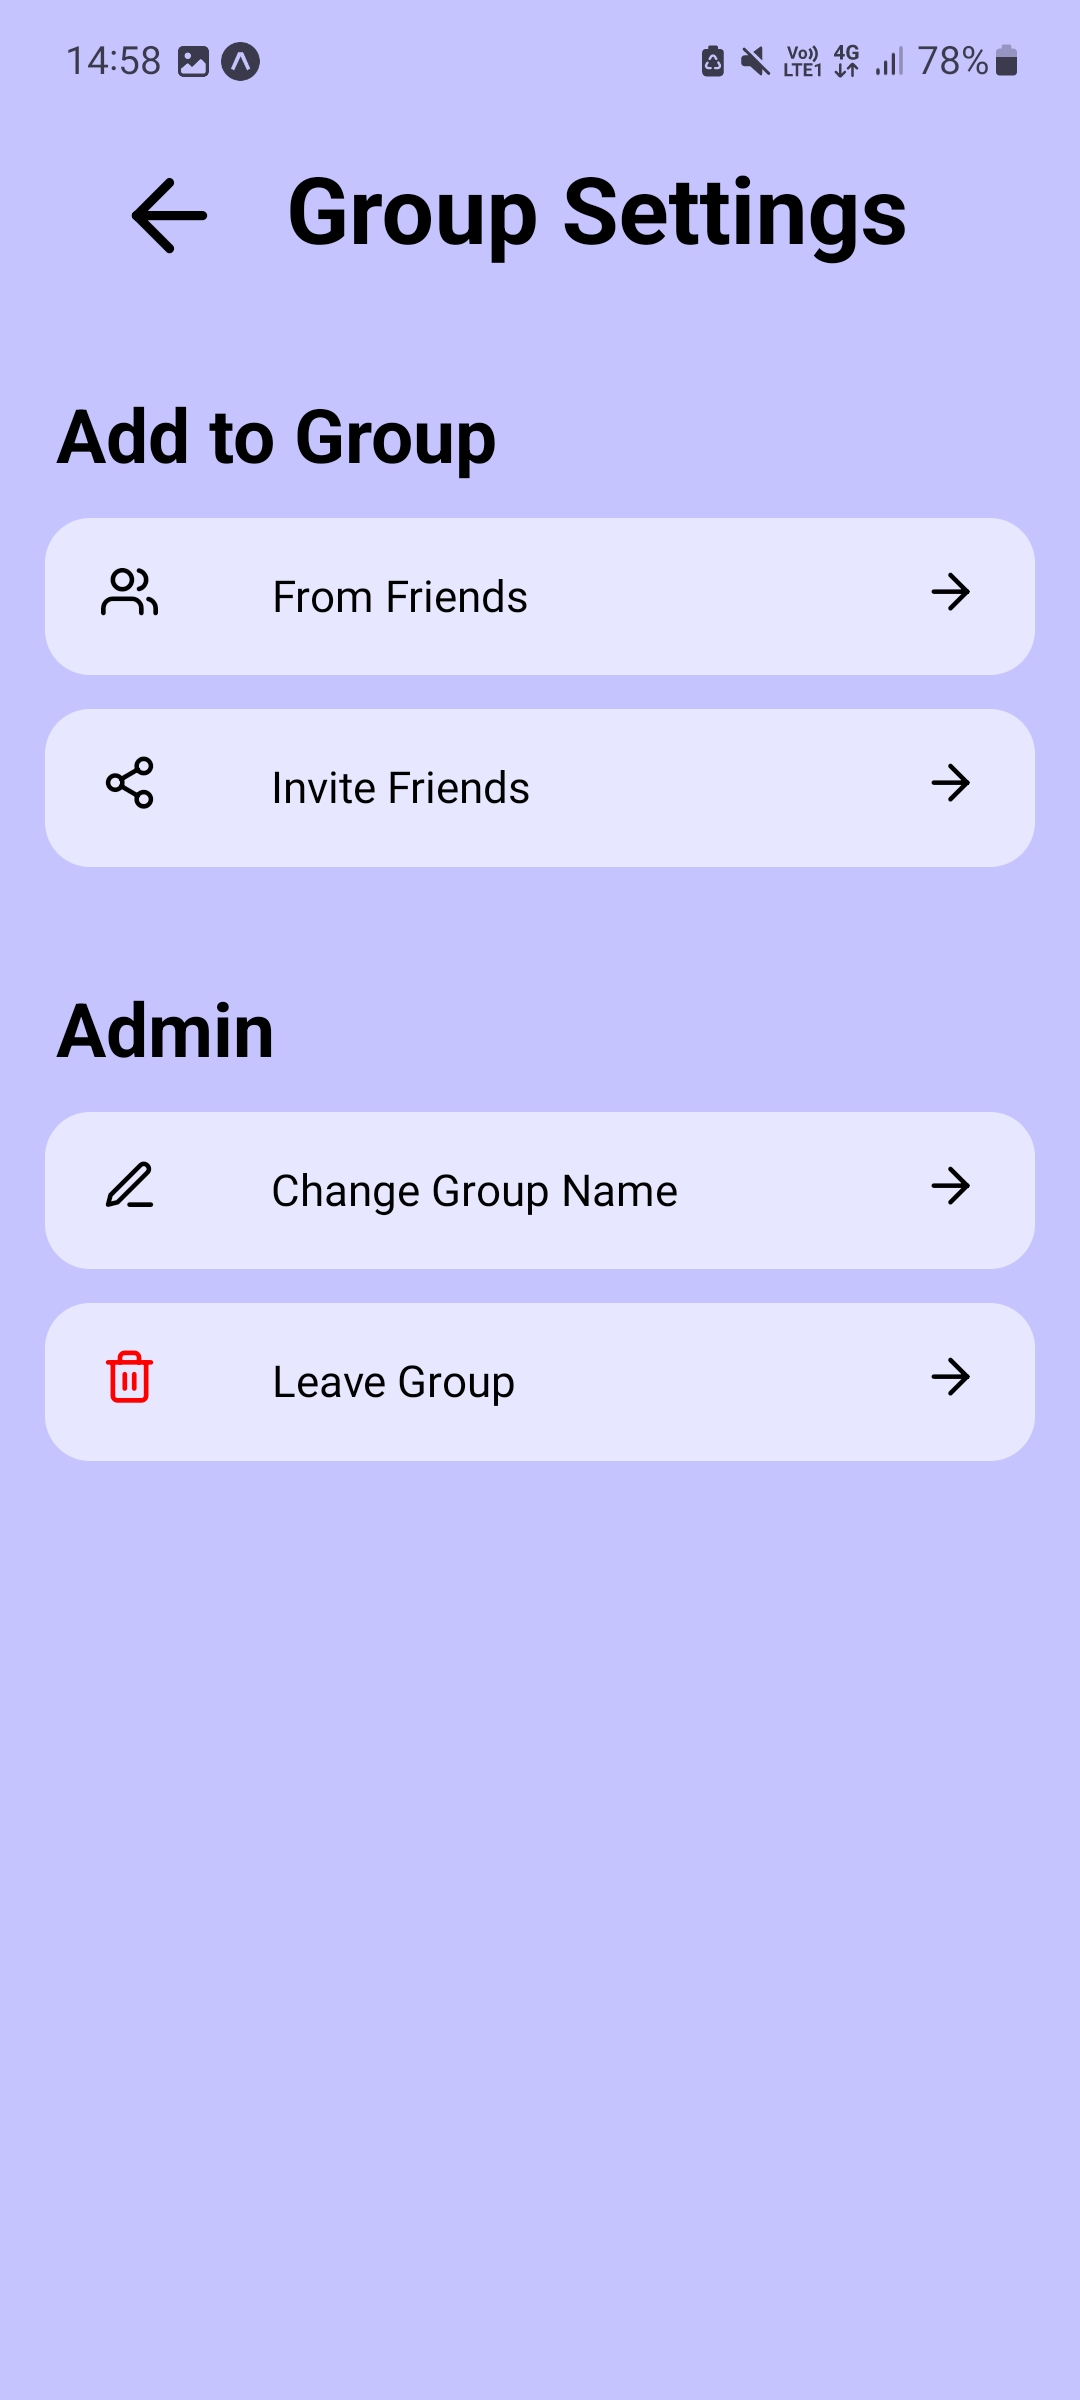
\includegraphics[width=\textwidth]{groupSettings.jpg}}
        \caption{Group Settings}
    \end{subfigure}
    \hspace{0.5em}
    \noindent\begin{subfigure}[b]{0.23\textwidth}
        \centering
        \frame{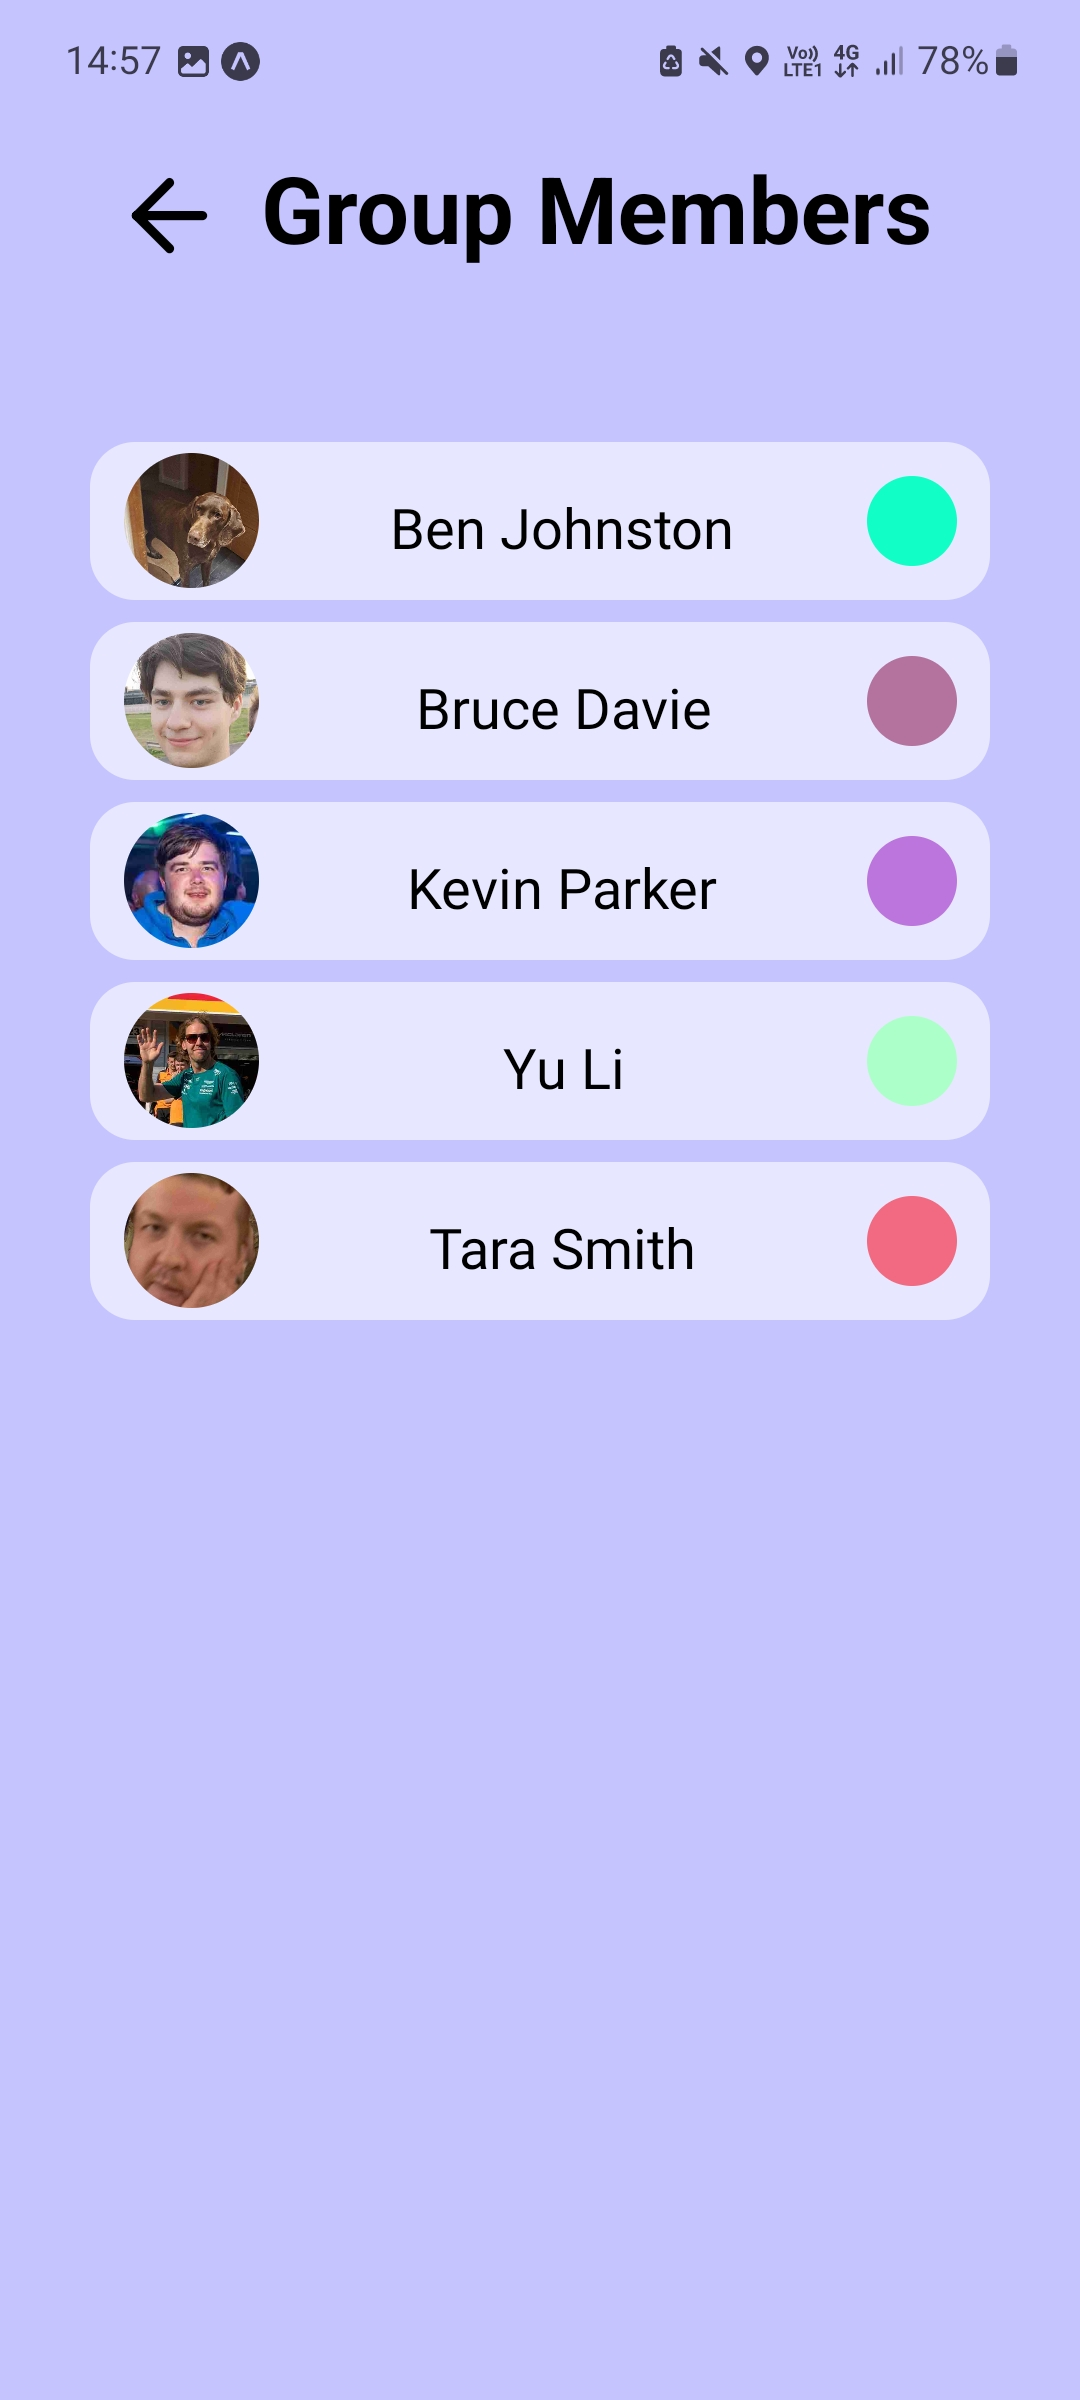
\includegraphics[width=\textwidth]{groupMembers.jpg}}
        \caption{Group Members}
    \end{subfigure}
    \vskip\baselineskip
    \noindent\begin{subfigure}[b]{0.23\textwidth}
        \centering
        \frame{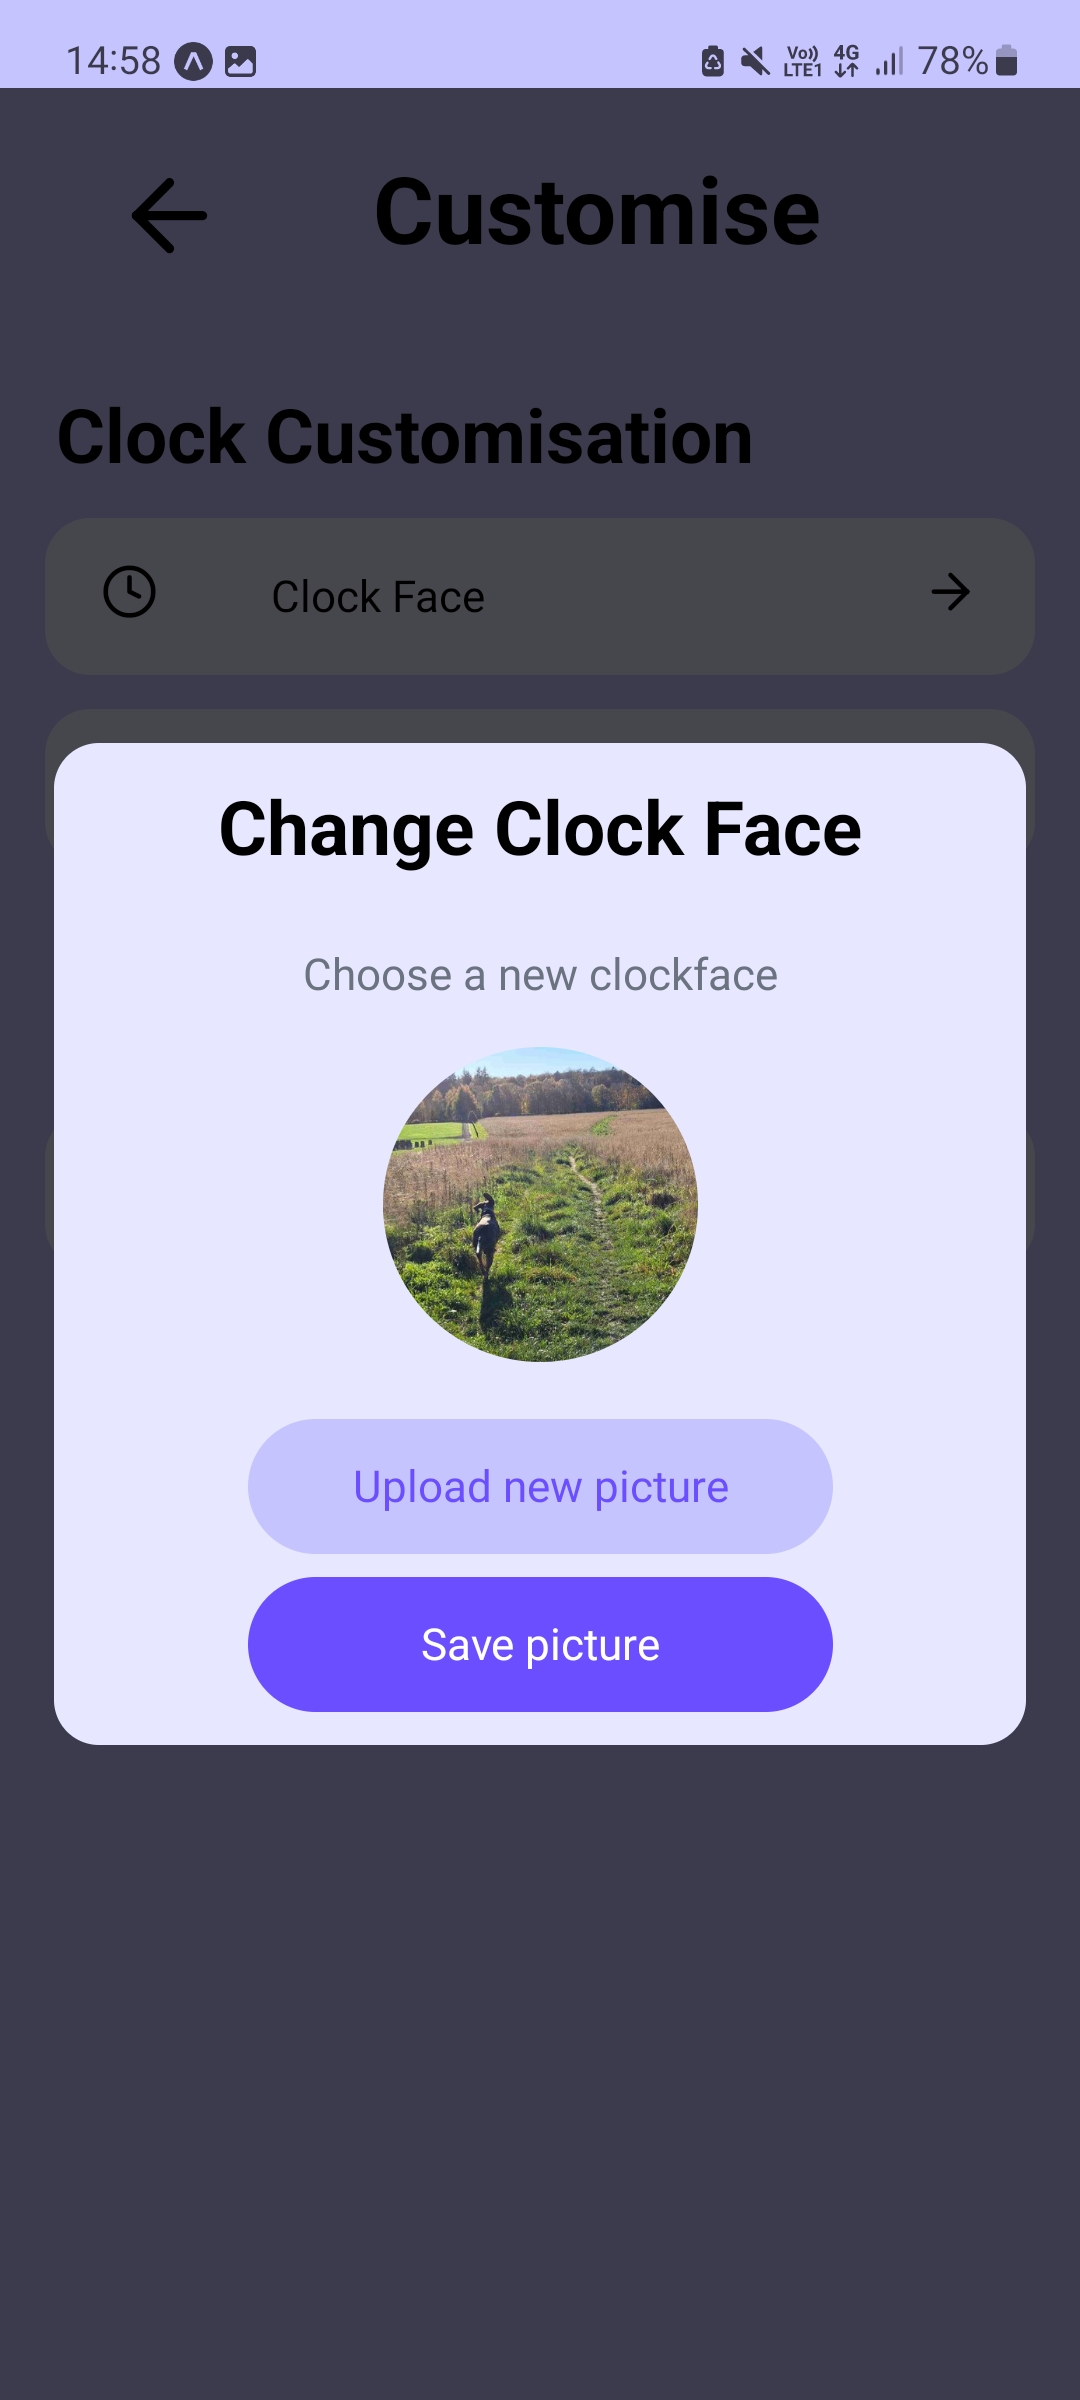
\includegraphics[width=\textwidth]{clockImg.jpg}}
        \caption{Clock Image Upload}
    \end{subfigure}
    \hspace{0.5em}
    \noindent\begin{subfigure}[b]{0.23\textwidth}
        \centering
        \frame{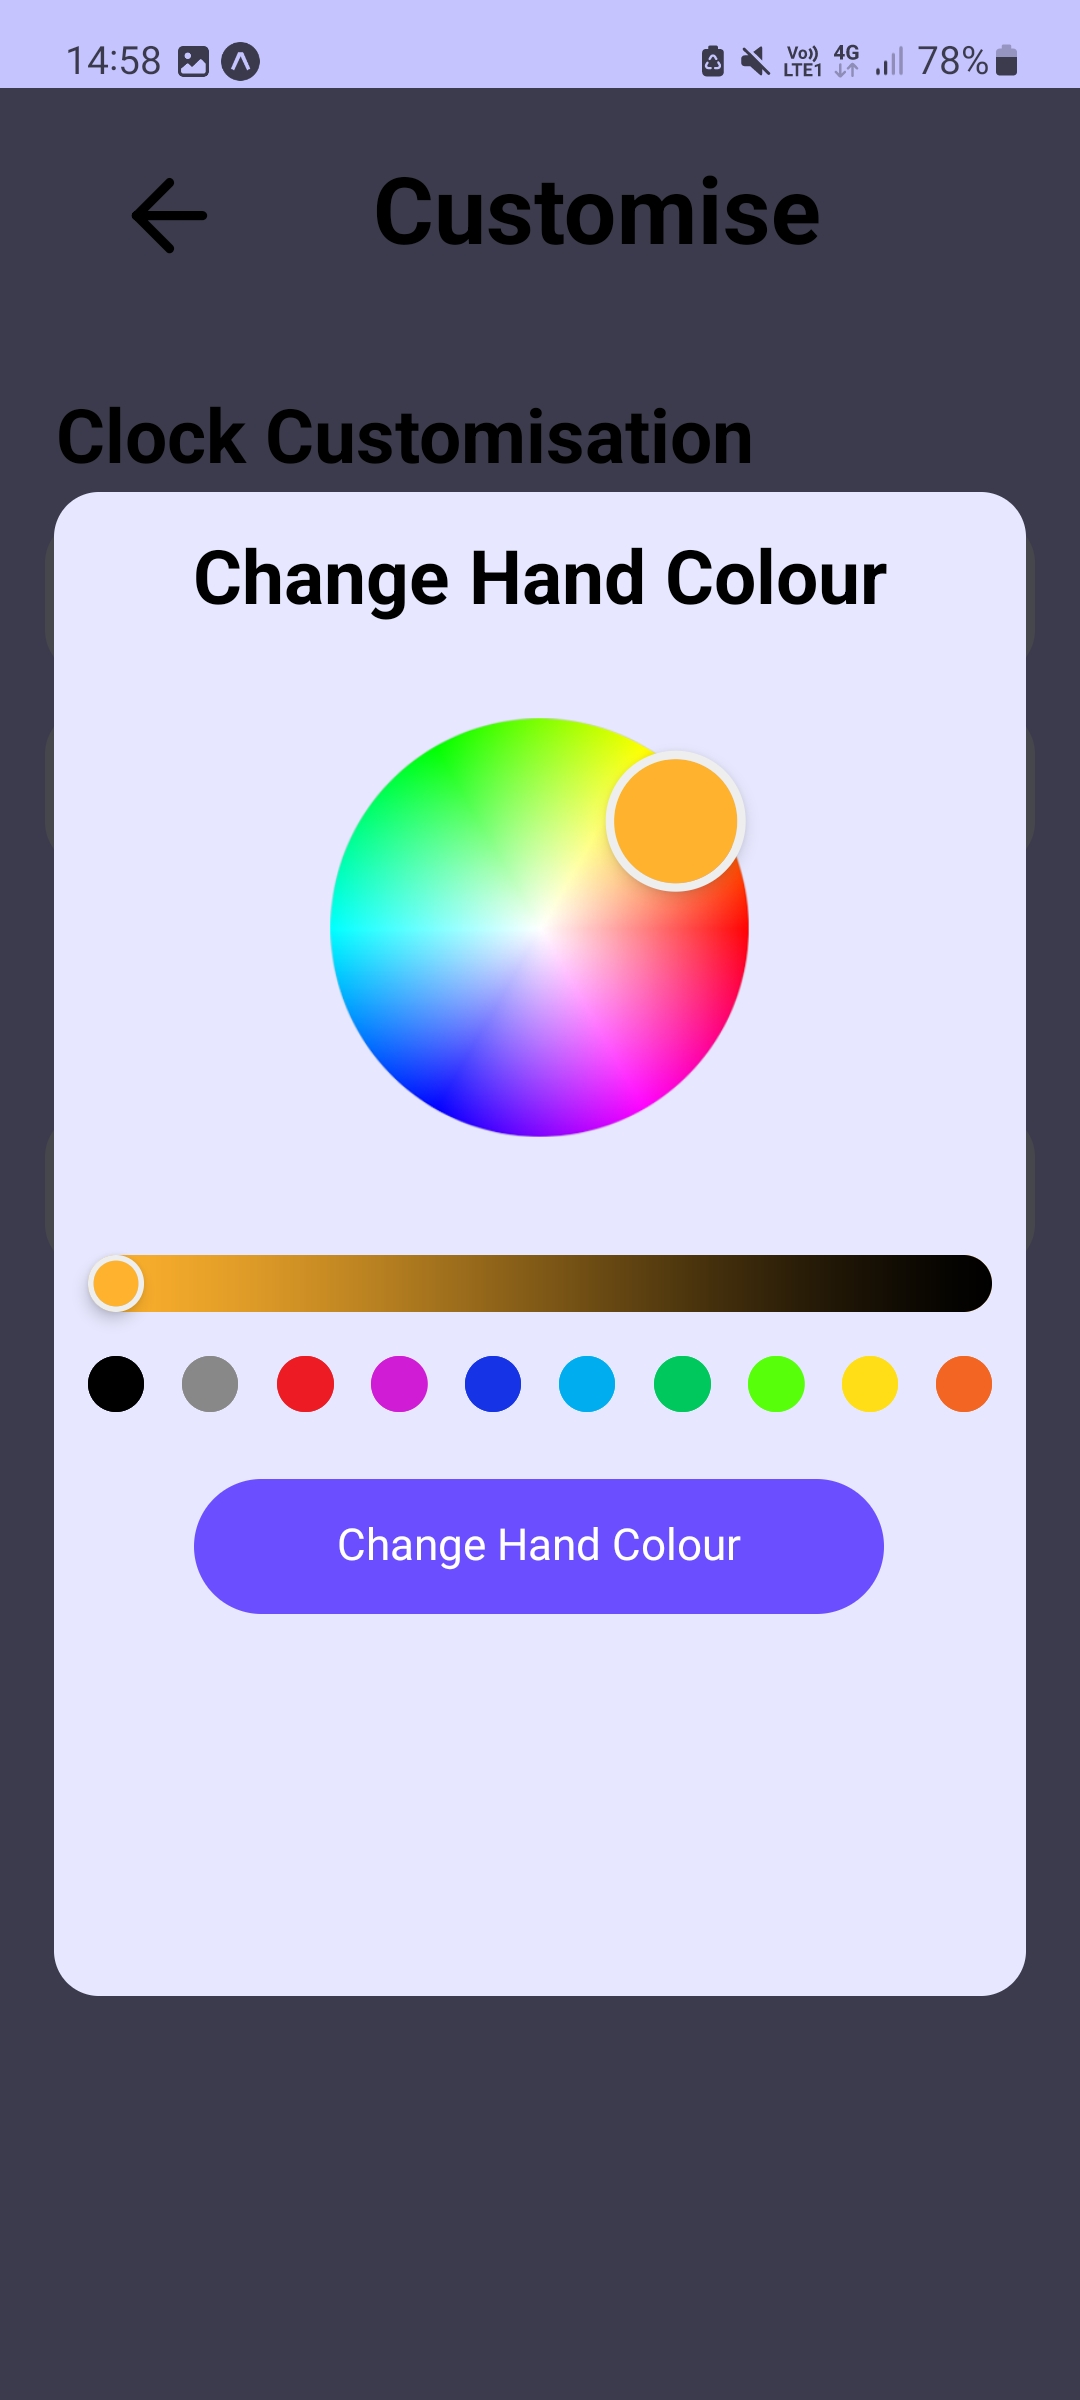
\includegraphics[width=\textwidth]{handCol.jpg}}
        \caption{Hand Colour Change}
    \end{subfigure}
    \hspace{0.5em}
    \noindent\begin{subfigure}[b]{0.23\textwidth}
        \centering
        \frame{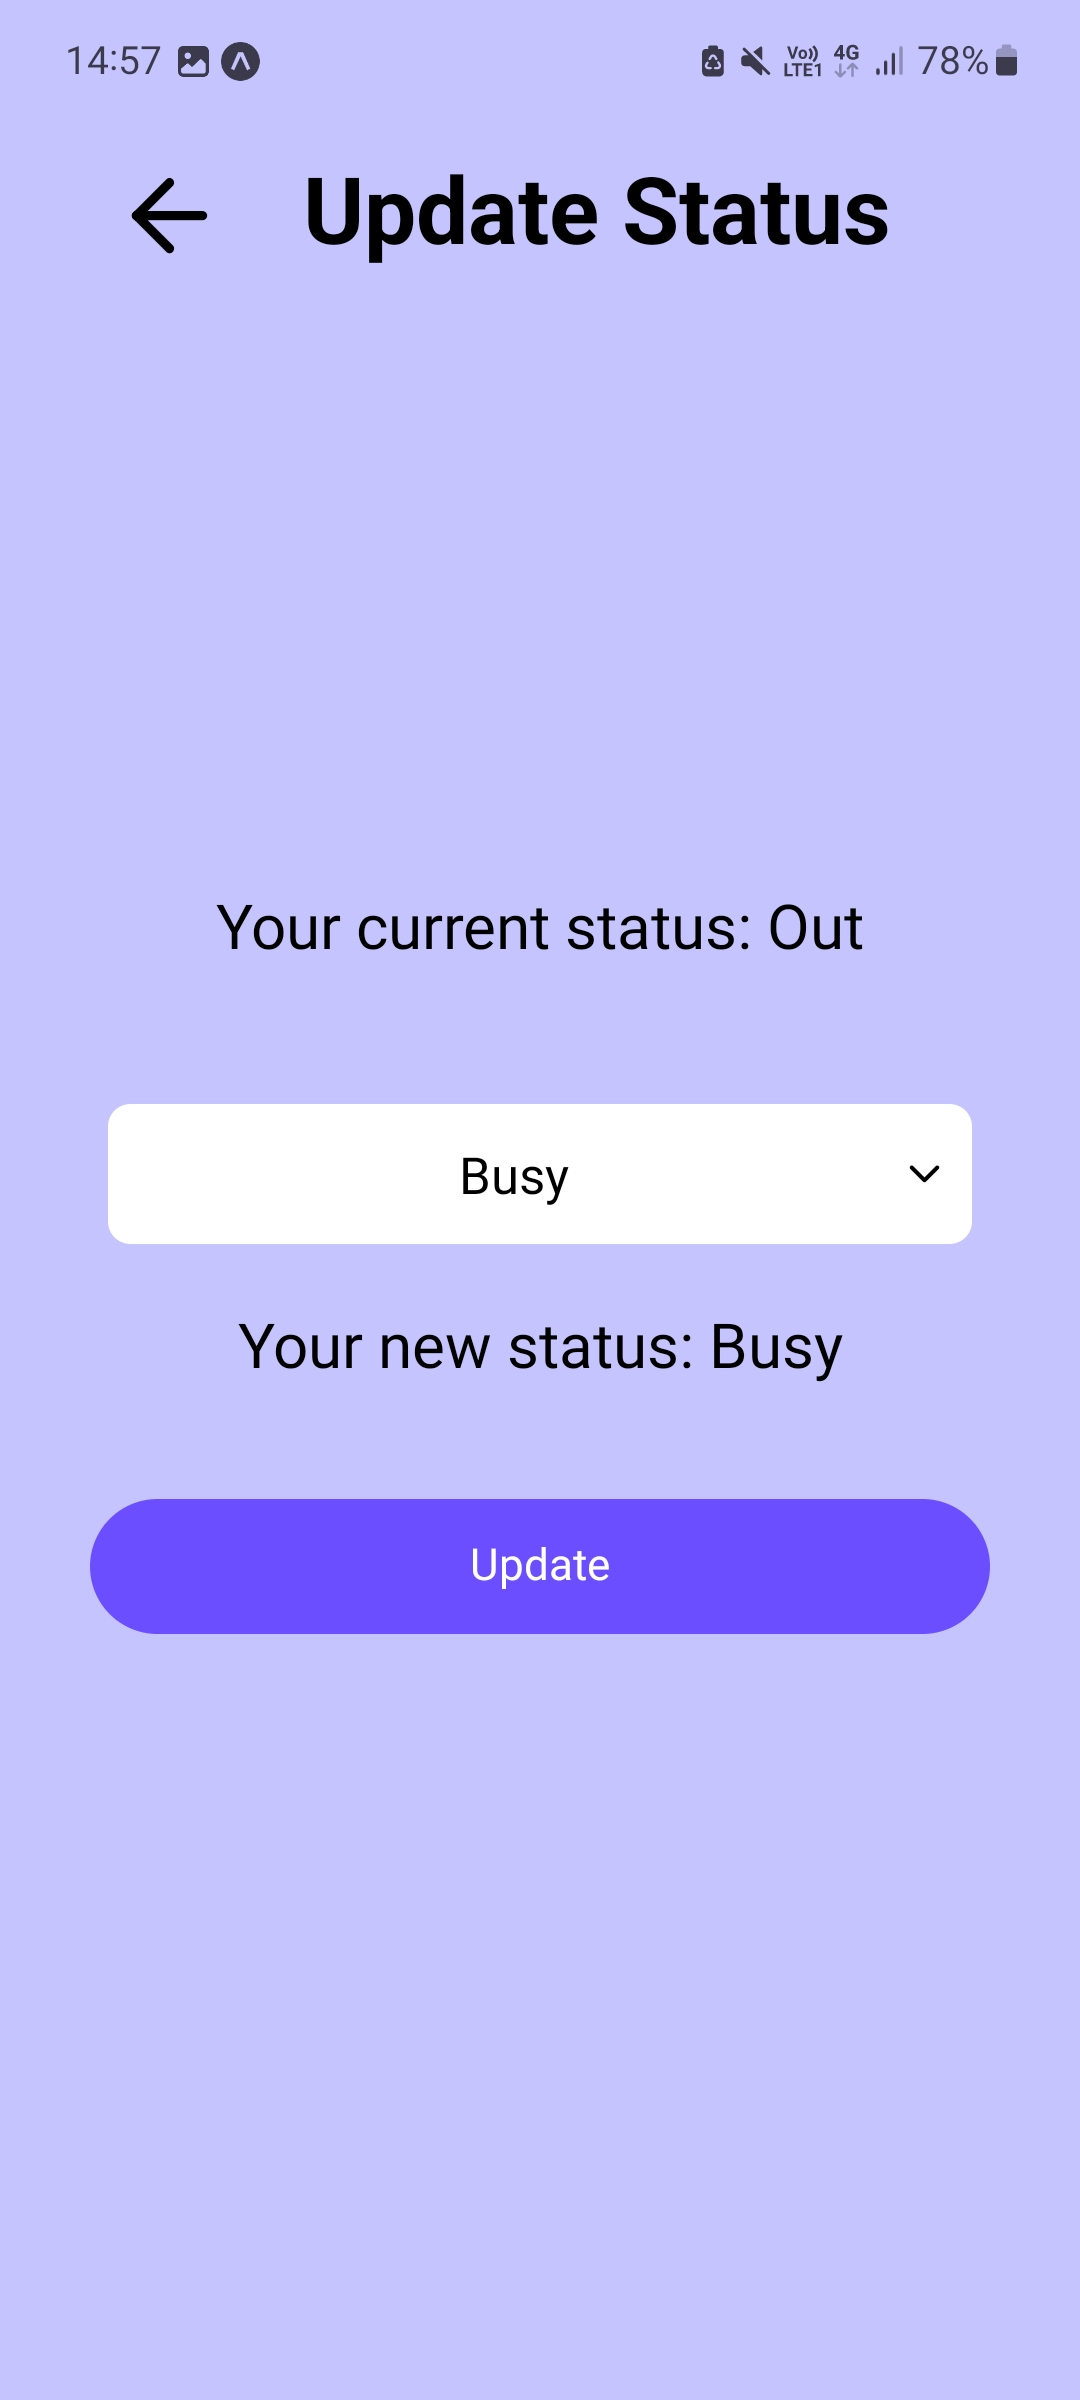
\includegraphics[width=\textwidth]{updateStat.jpg}}
        \caption{Update Status}
    \end{subfigure}
    \hspace{0.5em}
    \noindent\begin{subfigure}[b]{0.23\textwidth}
        \centering
        \frame{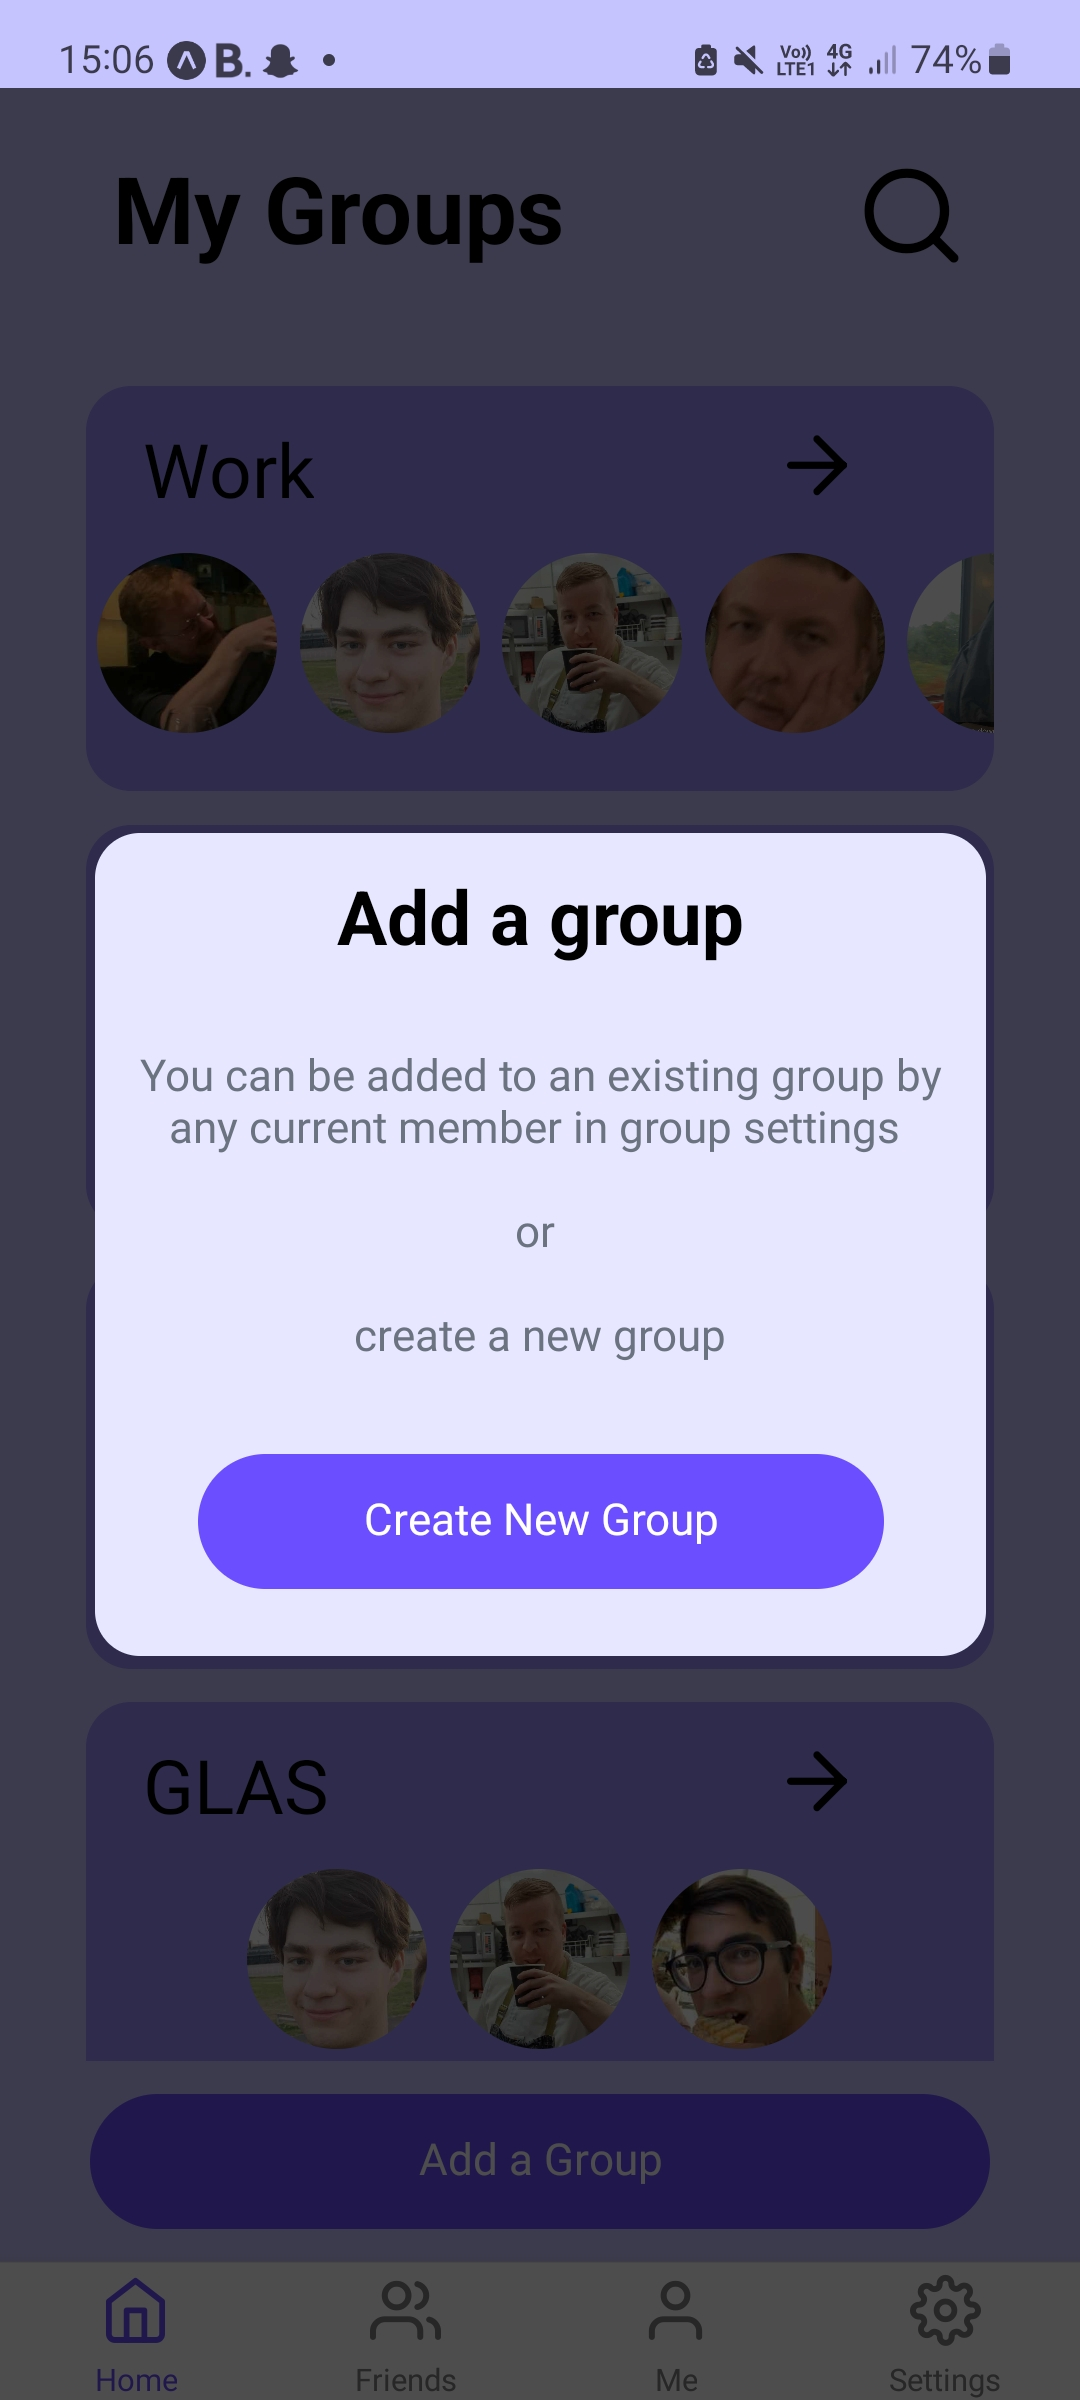
\includegraphics[width=\textwidth]{addGroup.jpg}}
        \caption{Add Group}
    \end{subfigure}
    \caption{Application pages}
\end{figure}
\FloatBarrier

\section{Reusable Component}\label{appendix:reusable}
\begin{figure}[!htbp]
    \centering
    \begin{subfigure}[b]{0.9\textwidth}
        \begin{lstlisting}[language=jsJsx]
        function AppButtonPurple(props) {
          const { title, onPressFunct } = props;
          return (
            <TouchableOpacity
              onPress={onPressFunct}
              className="bg-darkerPurple h-12 w-10/12 pt-3 rounded-full mx-1.5"
            >
              <Text className="text-white text-center">{title}</Text>
            </TouchableOpacity>
          );
        }
        
        AppButtonPurple.propTypes = {
          title: PropTypes.string.isRequired,
          onPressFunct: PropTypes.func.isRequired,
        };
        \end{lstlisting}
    \end{subfigure}
    \caption{Example of a reusable component}
    \small\textit{Here an onPress function and title are passed to this component to create a purple button with this title and onPress functionality. }
    \label{fig:tailwind}
\end{figure}
\FloatBarrier

\section{Realtime database overview}\label{appendix:rtdb}
\begin{figure}[!htbp]
    \centering
    \begin{subfigure}[b]{\textwidth}
        \frame{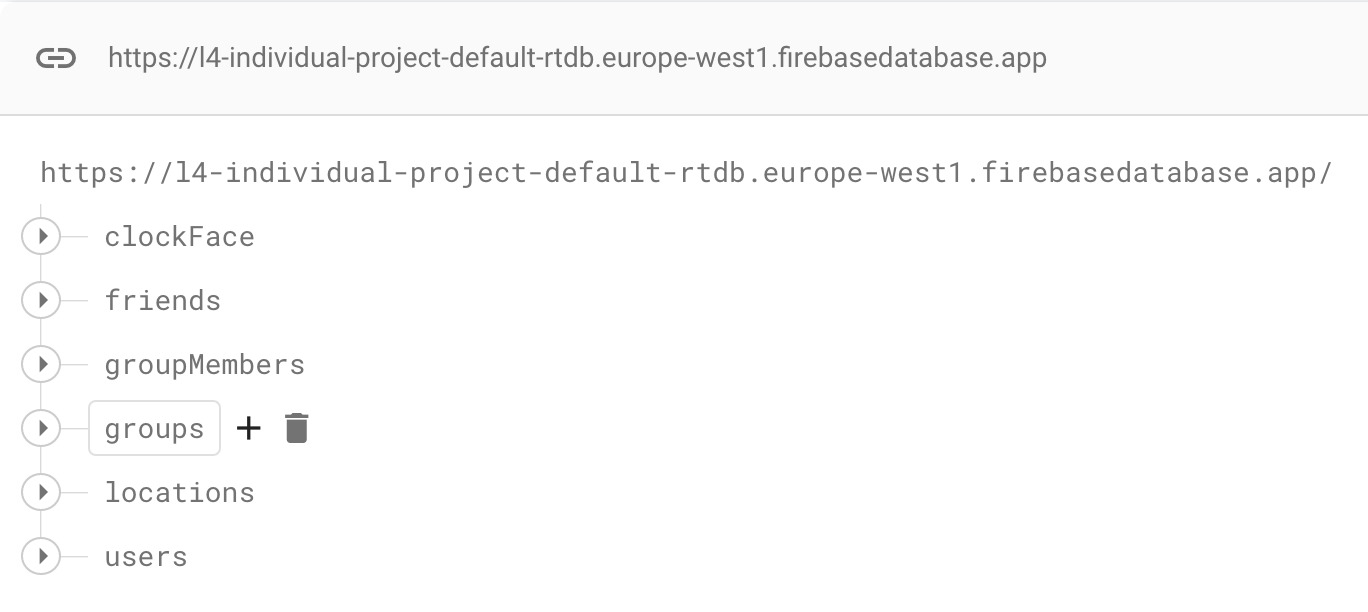
\includegraphics[width=\textwidth]{rtdb.png}}
    \end{subfigure}
    \caption{The JSON tree for the applications realtime database}
\end{figure}
\FloatBarrier
\newpage

\section{Realtime database security rules}\label{appendix:securityRulesRTDB}
\begin{figure}[!htbp]
    \centering
    \begin{subfigure}[b]{0.6\textwidth}
        \frame{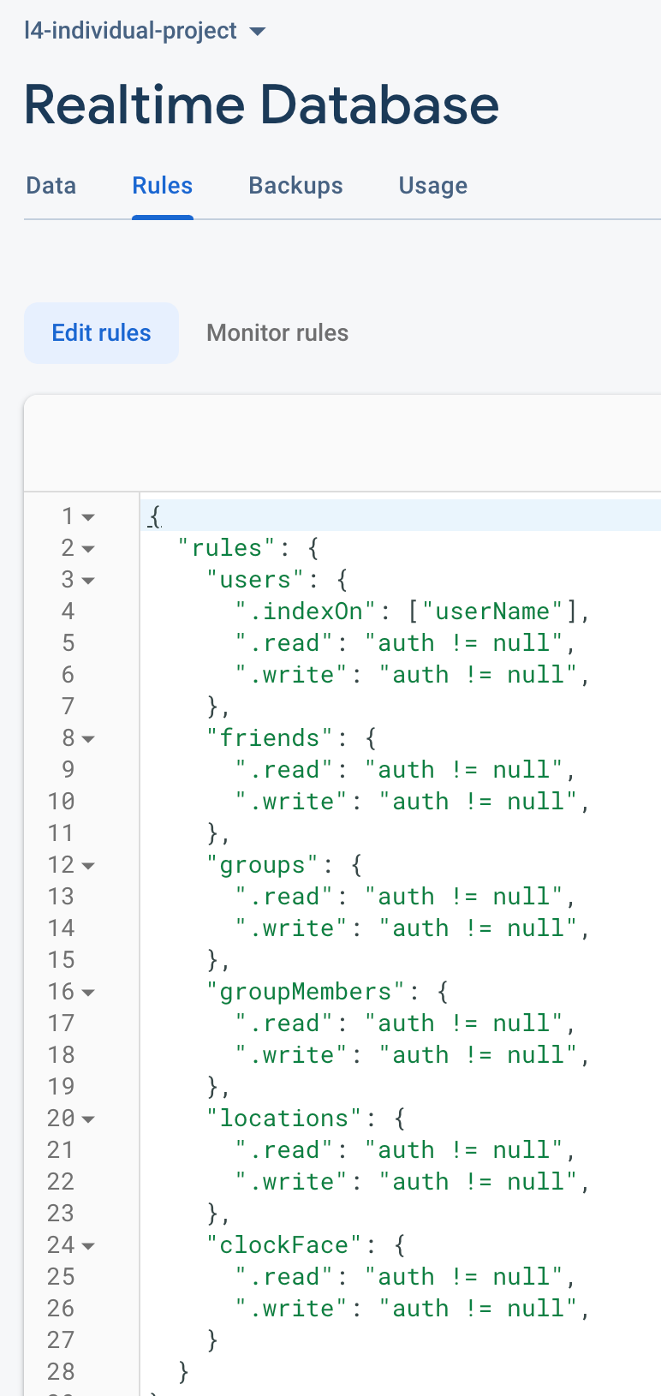
\includegraphics[width=\textwidth]{securityRulesRTDB.png}}
    \end{subfigure}
    \caption{The security rules for the realtime database}
    \small\textit{Here only authenticated users can read, or, write to the database}
\end{figure}
\FloatBarrier
\newpage

\section{Storage security rules}\label{appendix:securityRulesStor}
\begin{figure}[!htbp]
    \centering
    \begin{subfigure}[b]{0.8\textwidth}
        \frame{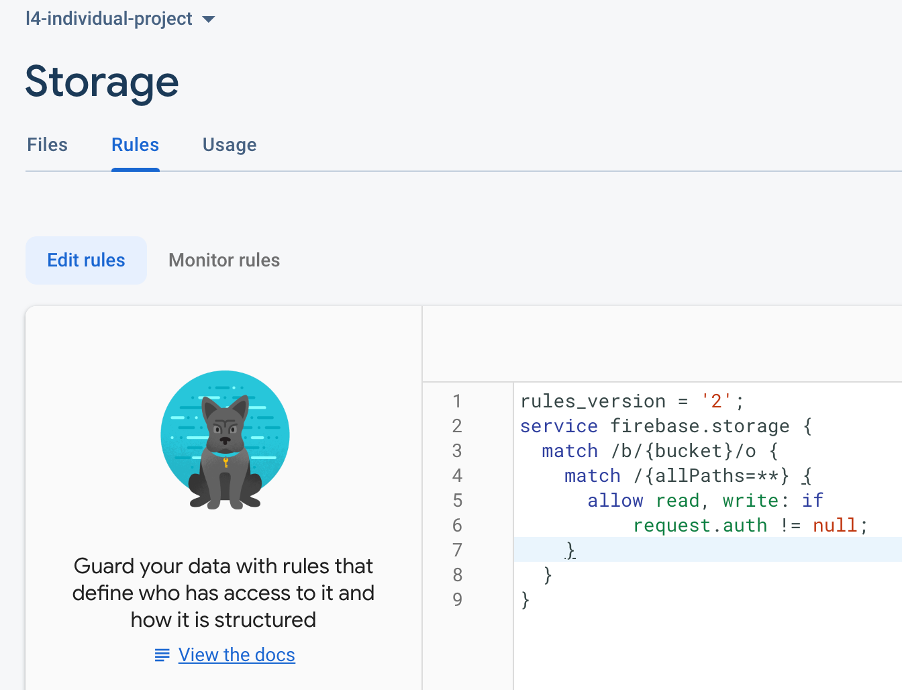
\includegraphics[width=\textwidth]{securityRulesStor.png}}
    \end{subfigure}
    \caption{The security rules for the cloud storage}
    \small\textit{Here only authenticated users can read, or, write to the storage}
\end{figure}
\FloatBarrier